\documentclass[twoside]{book}

% Packages required by doxygen
\usepackage{fixltx2e}
\usepackage{calc}
\usepackage{doxygen}
\usepackage[export]{adjustbox} % also loads graphicx
\usepackage{graphicx}
\usepackage[utf8]{inputenc}
\usepackage{makeidx}
\usepackage{multicol}
\usepackage{multirow}
\PassOptionsToPackage{warn}{textcomp}
\usepackage{textcomp}
\usepackage[nointegrals]{wasysym}
\usepackage[table]{xcolor}

% Font selection
\usepackage[T1]{fontenc}
\usepackage[scaled=.90]{helvet}
\usepackage{courier}
\usepackage{amssymb}
\usepackage{sectsty}
\renewcommand{\familydefault}{\sfdefault}
\allsectionsfont{%
  \fontseries{bc}\selectfont%
  \color{darkgray}%
}
\renewcommand{\DoxyLabelFont}{%
  \fontseries{bc}\selectfont%
  \color{darkgray}%
}
\newcommand{\+}{\discretionary{\mbox{\scriptsize$\hookleftarrow$}}{}{}}

% Page & text layout
\usepackage{geometry}
\geometry{%
  a4paper,%
  top=2.5cm,%
  bottom=2.5cm,%
  left=2.5cm,%
  right=2.5cm%
}
\tolerance=750
\hfuzz=15pt
\hbadness=750
\setlength{\emergencystretch}{15pt}
\setlength{\parindent}{0cm}
\setlength{\parskip}{3ex plus 2ex minus 2ex}
\makeatletter
\renewcommand{\paragraph}{%
  \@startsection{paragraph}{4}{0ex}{-1.0ex}{1.0ex}{%
    \normalfont\normalsize\bfseries\SS@parafont%
  }%
}
\renewcommand{\subparagraph}{%
  \@startsection{subparagraph}{5}{0ex}{-1.0ex}{1.0ex}{%
    \normalfont\normalsize\bfseries\SS@subparafont%
  }%
}
\makeatother

% Headers & footers
\usepackage{fancyhdr}
\pagestyle{fancyplain}
\fancyhead[LE]{\fancyplain{}{\bfseries\thepage}}
\fancyhead[CE]{\fancyplain{}{}}
\fancyhead[RE]{\fancyplain{}{\bfseries\leftmark}}
\fancyhead[LO]{\fancyplain{}{\bfseries\rightmark}}
\fancyhead[CO]{\fancyplain{}{}}
\fancyhead[RO]{\fancyplain{}{\bfseries\thepage}}
\fancyfoot[LE]{\fancyplain{}{}}
\fancyfoot[CE]{\fancyplain{}{}}
\fancyfoot[RE]{\fancyplain{}{\bfseries\scriptsize Generated by Doxygen }}
\fancyfoot[LO]{\fancyplain{}{\bfseries\scriptsize Generated by Doxygen }}
\fancyfoot[CO]{\fancyplain{}{}}
\fancyfoot[RO]{\fancyplain{}{}}
\renewcommand{\footrulewidth}{0.4pt}
\renewcommand{\chaptermark}[1]{%
  \markboth{#1}{}%
}
\renewcommand{\sectionmark}[1]{%
  \markright{\thesection\ #1}%
}

% Indices & bibliography
\usepackage{natbib}
\usepackage[titles]{tocloft}
\setcounter{tocdepth}{3}
\setcounter{secnumdepth}{5}
\makeindex

% Hyperlinks (required, but should be loaded last)
\usepackage{ifpdf}
\ifpdf
  \usepackage[pdftex,pagebackref=true]{hyperref}
\else
  \usepackage[ps2pdf,pagebackref=true]{hyperref}
\fi
\hypersetup{%
  colorlinks=true,%
  linkcolor=blue,%
  citecolor=blue,%
  unicode%
}

% Custom commands
\newcommand{\clearemptydoublepage}{%
  \newpage{\pagestyle{empty}\cleardoublepage}%
}

\usepackage{caption}
\captionsetup{labelsep=space,justification=centering,font={bf},singlelinecheck=off,skip=4pt,position=top}

%===== C O N T E N T S =====

\begin{document}

% Titlepage & ToC
\hypersetup{pageanchor=false,
             bookmarksnumbered=true,
             pdfencoding=unicode
            }
\pagenumbering{roman}
\begin{titlepage}
\vspace*{7cm}
\begin{center}%
{\Large G1\+\_\+\+Brizon\+\_\+\+Cartier\+\_\+\+De\+La\+Fuente\+\_\+\+Roda }\\
\vspace*{1cm}
{\large Generated by Doxygen 1.8.11}\\
\end{center}
\end{titlepage}
\clearemptydoublepage
\tableofcontents
\clearemptydoublepage
\pagenumbering{arabic}
\hypersetup{pageanchor=true}

%--- Begin generated contents ---
\chapter{Class Index}
\section{Class List}
Here are the classes, structs, unions and interfaces with brief descriptions\+:\begin{DoxyCompactList}
\item\contentsline{section}{\hyperlink{struct_c_my_param}{C\+My\+Param} }{\pageref{struct_c_my_param}}{}
\item\contentsline{section}{\hyperlink{struct_structure}{Structure} }{\pageref{struct_structure}}{}
\end{DoxyCompactList}

\chapter{File Index}
\section{File List}
Here is a list of all files with brief descriptions\+:\begin{DoxyCompactList}
\item\contentsline{section}{/home/jyroda/\+Documents/\+G1\+\_\+\+Brizon\+\_\+\+Cartier\+\_\+\+De\+La\+Fuente\+\_\+\+Roda/\hyperlink{main_8cpp}{main.\+cpp} \\*Terminal\textquotesingle{}s color management beginning of the project titled \char`\"{}catch me if you can\char`\"{} }{\pageref{main_8cpp}}{}
\end{DoxyCompactList}

\chapter{Class Documentation}
\hypertarget{struct_c_my_param}{}\section{C\+My\+Param Struct Reference}
\label{struct_c_my_param}\index{C\+My\+Param@{C\+My\+Param}}
\subsection*{Public Attributes}
\begin{DoxyCompactItemize}
\item 
map$<$ string, char $>$ \hyperlink{struct_c_my_param_ac8cbc4799636b69d4a1262671c7d6b6d}{Controls}
\item 
char \hyperlink{struct_c_my_param_a4df5fa144f6e427e038fac7fbd28e6d7}{food}
\item 
map$<$ string, string $>$ \hyperlink{struct_c_my_param_a5d421abb0e990e5845f6257452b08612}{Colors}
\item 
map$<$ string, string $>$ \hyperlink{struct_c_my_param_a14680b6b2da1e5d7d4c580d290bd1d4b}{Game\+Strings}
\item 
bool \hyperlink{struct_c_my_param_a56420b1ed8e44615fd5ae20c86ba7a6c}{IA}
\item 
unsigned \hyperlink{struct_c_my_param_a3848248ca913f8abff022ca7e9de4219}{difficulty}
\item 
unsigned \hyperlink{struct_c_my_param_a7492c88f87a6eb26f15c7e4008c38519}{random\+Frequency}
\item 
unsigned \hyperlink{struct_c_my_param_a3afeb99110158c6cf4d68ad5246f0043}{end\+Time}
\end{DoxyCompactItemize}


\subsection{Member Data Documentation}
\index{C\+My\+Param@{C\+My\+Param}!Colors@{Colors}}
\index{Colors@{Colors}!C\+My\+Param@{C\+My\+Param}}
\subsubsection[{\texorpdfstring{Colors}{Colors}}]{\setlength{\rightskip}{0pt plus 5cm}map$<$string, string$>$ C\+My\+Param\+::\+Colors}\hypertarget{struct_c_my_param_a5d421abb0e990e5845f6257452b08612}{}\label{struct_c_my_param_a5d421abb0e990e5845f6257452b08612}
\index{C\+My\+Param@{C\+My\+Param}!Controls@{Controls}}
\index{Controls@{Controls}!C\+My\+Param@{C\+My\+Param}}
\subsubsection[{\texorpdfstring{Controls}{Controls}}]{\setlength{\rightskip}{0pt plus 5cm}map$<$string, char$>$ C\+My\+Param\+::\+Controls}\hypertarget{struct_c_my_param_ac8cbc4799636b69d4a1262671c7d6b6d}{}\label{struct_c_my_param_ac8cbc4799636b69d4a1262671c7d6b6d}
\index{C\+My\+Param@{C\+My\+Param}!difficulty@{difficulty}}
\index{difficulty@{difficulty}!C\+My\+Param@{C\+My\+Param}}
\subsubsection[{\texorpdfstring{difficulty}{difficulty}}]{\setlength{\rightskip}{0pt plus 5cm}unsigned C\+My\+Param\+::difficulty}\hypertarget{struct_c_my_param_a3848248ca913f8abff022ca7e9de4219}{}\label{struct_c_my_param_a3848248ca913f8abff022ca7e9de4219}
\index{C\+My\+Param@{C\+My\+Param}!end\+Time@{end\+Time}}
\index{end\+Time@{end\+Time}!C\+My\+Param@{C\+My\+Param}}
\subsubsection[{\texorpdfstring{end\+Time}{endTime}}]{\setlength{\rightskip}{0pt plus 5cm}unsigned C\+My\+Param\+::end\+Time}\hypertarget{struct_c_my_param_a3afeb99110158c6cf4d68ad5246f0043}{}\label{struct_c_my_param_a3afeb99110158c6cf4d68ad5246f0043}
\index{C\+My\+Param@{C\+My\+Param}!food@{food}}
\index{food@{food}!C\+My\+Param@{C\+My\+Param}}
\subsubsection[{\texorpdfstring{food}{food}}]{\setlength{\rightskip}{0pt plus 5cm}char C\+My\+Param\+::food}\hypertarget{struct_c_my_param_a4df5fa144f6e427e038fac7fbd28e6d7}{}\label{struct_c_my_param_a4df5fa144f6e427e038fac7fbd28e6d7}
\index{C\+My\+Param@{C\+My\+Param}!Game\+Strings@{Game\+Strings}}
\index{Game\+Strings@{Game\+Strings}!C\+My\+Param@{C\+My\+Param}}
\subsubsection[{\texorpdfstring{Game\+Strings}{GameStrings}}]{\setlength{\rightskip}{0pt plus 5cm}map$<$string, string$>$ C\+My\+Param\+::\+Game\+Strings}\hypertarget{struct_c_my_param_a14680b6b2da1e5d7d4c580d290bd1d4b}{}\label{struct_c_my_param_a14680b6b2da1e5d7d4c580d290bd1d4b}
\index{C\+My\+Param@{C\+My\+Param}!IA@{IA}}
\index{IA@{IA}!C\+My\+Param@{C\+My\+Param}}
\subsubsection[{\texorpdfstring{IA}{IA}}]{\setlength{\rightskip}{0pt plus 5cm}bool C\+My\+Param\+::\+IA}\hypertarget{struct_c_my_param_a56420b1ed8e44615fd5ae20c86ba7a6c}{}\label{struct_c_my_param_a56420b1ed8e44615fd5ae20c86ba7a6c}
\index{C\+My\+Param@{C\+My\+Param}!random\+Frequency@{random\+Frequency}}
\index{random\+Frequency@{random\+Frequency}!C\+My\+Param@{C\+My\+Param}}
\subsubsection[{\texorpdfstring{random\+Frequency}{randomFrequency}}]{\setlength{\rightskip}{0pt plus 5cm}unsigned C\+My\+Param\+::random\+Frequency}\hypertarget{struct_c_my_param_a7492c88f87a6eb26f15c7e4008c38519}{}\label{struct_c_my_param_a7492c88f87a6eb26f15c7e4008c38519}


The documentation for this struct was generated from the following file\+:\begin{DoxyCompactItemize}
\item 
/home/jyroda/\+Documents/\+G1\+\_\+\+Brizon\+\_\+\+Cartier\+\_\+\+De\+La\+Fuente\+\_\+\+Roda/\hyperlink{main_8cpp}{main.\+cpp}\end{DoxyCompactItemize}

\hypertarget{struct_structure}{}\section{Structure Struct Reference}
\label{struct_structure}\index{Structure@{Structure}}


\subsection{Detailed Description}
parametres du jeu 

The documentation for this struct was generated from the following file\+:\begin{DoxyCompactItemize}
\item 
/home/jyroda/\+Documents/\+G1\+\_\+\+Brizon\+\_\+\+Cartier\+\_\+\+De\+La\+Fuente\+\_\+\+Roda/\hyperlink{main_8cpp}{main.\+cpp}\end{DoxyCompactItemize}

\chapter{File Documentation}
\hypertarget{main_8cpp}{}\section{/home/jyroda/\+Documents/\+G1\+\_\+\+Brizon\+\_\+\+Cartier\+\_\+\+De\+La\+Fuente\+\_\+\+Roda/main.cpp File Reference}
\label{main_8cpp}\index{/home/jyroda/\+Documents/\+G1\+\_\+\+Brizon\+\_\+\+Cartier\+\_\+\+De\+La\+Fuente\+\_\+\+Roda/main.\+cpp@{/home/jyroda/\+Documents/\+G1\+\_\+\+Brizon\+\_\+\+Cartier\+\_\+\+De\+La\+Fuente\+\_\+\+Roda/main.\+cpp}}


Terminal\textquotesingle{}s color management beginning of the project titled \char`\"{}catch me if you can\char`\"{}.  


{\ttfamily \#include $<$iostream$>$}\\*
{\ttfamily \#include $<$istream$>$}\\*
{\ttfamily \#include $<$vector$>$}\\*
{\ttfamily \#include $<$sys/ioctl.\+h$>$}\\*
{\ttfamily \#include $<$unistd.\+h$>$}\\*
{\ttfamily \#include $<$termios.\+h$>$}\\*
{\ttfamily \#include $<$time.\+h$>$}\\*
{\ttfamily \#include $<$dirent.\+h$>$}\\*
{\ttfamily \#include $<$stdio.\+h$>$}\\*
{\ttfamily \#include $<$random$>$}\\*
{\ttfamily \#include $<$fstream$>$}\\*
{\ttfamily \#include $<$iomanip$>$}\\*
{\ttfamily \#include $<$string$>$}\\*
{\ttfamily \#include $<$map$>$}\\*
{\ttfamily \#include $<$algorithm$>$}\\*
Include dependency graph for main.\+cpp\+:\nopagebreak
\begin{figure}[H]
\begin{center}
\leavevmode
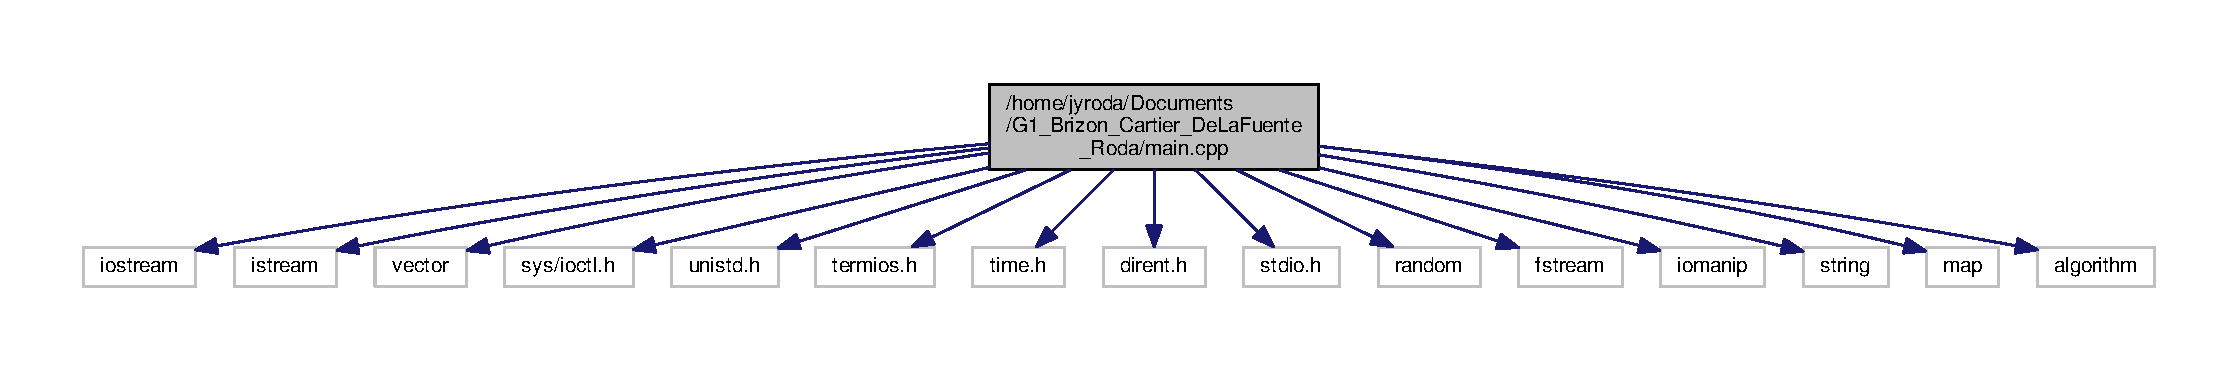
\includegraphics[width=350pt]{main_8cpp__incl}
\end{center}
\end{figure}
\subsection*{Classes}
\begin{DoxyCompactItemize}
\item 
struct \hyperlink{struct_c_my_param}{C\+My\+Param}
\end{DoxyCompactItemize}
\subsection*{Typedefs}
\begin{DoxyCompactItemize}
\item 
typedef vector$<$ char $>$ \hyperlink{main_8cpp_ad6fbcb1fd9b9432e05a0213cf65f33fc}{C\+V\+Line}
\begin{DoxyCompactList}\small\item\em Type représentant une ligne dans la grille du jeu. \end{DoxyCompactList}\item 
typedef vector$<$ \hyperlink{main_8cpp_ad6fbcb1fd9b9432e05a0213cf65f33fc}{C\+V\+Line} $>$ \hyperlink{main_8cpp_a090413f30f1a2687e1fb4532555b1f90}{C\+Matrix}
\begin{DoxyCompactList}\small\item\em Type représentant la grille du jeu. \end{DoxyCompactList}\item 
typedef pair$<$ unsigned, unsigned $>$ \hyperlink{main_8cpp_a0a028f84cf0521f2c7ecf26d217e484e}{C\+Position}
\begin{DoxyCompactList}\small\item\em Type représentant la position d\textquotesingle{}un joueur dans la grille. \end{DoxyCompactList}\item 
typedef pair$<$ unsigned, unsigned $>$ \hyperlink{main_8cpp_a16e9343985d6496ab09abd0b60a9a8a7}{C\+Terminal\+Size}
\begin{DoxyCompactList}\small\item\em Type représentant la taille de la fenetre. \end{DoxyCompactList}\end{DoxyCompactItemize}
\subsection*{Functions}
\begin{DoxyCompactItemize}
\item 
const char \hyperlink{main_8cpp_a24d8d97414c569e372f4ff5c0a7e2fa0}{K\+Player\+Up} (\textquotesingle{}$^\wedge$\textquotesingle{})
\begin{DoxyCompactList}\small\item\em Joueur allant en haut. \end{DoxyCompactList}\item 
const char \hyperlink{main_8cpp_a9e68aa6a6900f7f9567ca2f689ae0bdc}{K\+Player\+Down} (\textquotesingle{}v\textquotesingle{})
\begin{DoxyCompactList}\small\item\em Joueur allant en bas. \end{DoxyCompactList}\item 
const char \hyperlink{main_8cpp_a0e0be1c05bbe1c9a11c01d5b8b558a70}{K\+Player\+Left} (\textquotesingle{}$<$\textquotesingle{})
\begin{DoxyCompactList}\small\item\em Joueur allant a gauche. \end{DoxyCompactList}\item 
const char \hyperlink{main_8cpp_acedb4c0046e67a1ce8618258be548e07}{K\+Player\+Right} (\textquotesingle{}$>$\textquotesingle{})
\begin{DoxyCompactList}\small\item\em Joueur allant à droite. \end{DoxyCompactList}\item 
const char \hyperlink{main_8cpp_a81a4a924185c81f623edfb38a4f629ed}{K\+Empty} (\textquotesingle{} \textquotesingle{})
\begin{DoxyCompactList}\small\item\em Espace vide. \end{DoxyCompactList}\item 
void \hyperlink{main_8cpp_a6a3ca153f0817e8ba91a023b886bb662}{Clear\+Screen} ()
\begin{DoxyCompactList}\small\item\em Efface l\textquotesingle{}écran du terminal. \end{DoxyCompactList}\item 
const string \hyperlink{main_8cpp_ae421976620c052c8350660039b8cb3bd}{K\+Reset} (\char`\"{}0\char`\"{})
\begin{DoxyCompactList}\small\item\em Code couleur nul (reinitialisation) \end{DoxyCompactList}\item 
const string \hyperlink{main_8cpp_a660c3e68e5967e553ae7fd9fb7073bbe}{K\+Noir} (\char`\"{}30\char`\"{})
\begin{DoxyCompactList}\small\item\em Code couleur noir. \end{DoxyCompactList}\item 
const string \hyperlink{main_8cpp_a09f08ffca2080e9ca9c050093a2ca6d5}{K\+Rouge} (\char`\"{}31\char`\"{})
\begin{DoxyCompactList}\small\item\em Code couleur rouge. \end{DoxyCompactList}\item 
const string \hyperlink{main_8cpp_a1cdcc3e3fe7660a6f85532bb0d228fee}{K\+Vert} (\char`\"{}32\char`\"{})
\begin{DoxyCompactList}\small\item\em Code couleur vert. \end{DoxyCompactList}\item 
const string \hyperlink{main_8cpp_af02736496532ff1e9c9137691bfb1e07}{K\+Jaune} (\char`\"{}33\char`\"{})
\begin{DoxyCompactList}\small\item\em Code couleur jaune. \end{DoxyCompactList}\item 
const string \hyperlink{main_8cpp_a566a648bad2891bdf1d5746fed6fc6d3}{K\+Bleu} (\char`\"{}34\char`\"{})
\begin{DoxyCompactList}\small\item\em Code couleur bleu. \end{DoxyCompactList}\item 
const string \hyperlink{main_8cpp_a0eb078e8b0f7aa0c81169197965bbdd2}{K\+M\+Agenta} (\char`\"{}35\char`\"{})
\begin{DoxyCompactList}\small\item\em Code couleur magenta. \end{DoxyCompactList}\item 
const string \hyperlink{main_8cpp_aa608863de5cd86b7b36f68a1189222cb}{K\+Cyan} (\char`\"{}36\char`\"{})
\begin{DoxyCompactList}\small\item\em Code couleur cyan. \end{DoxyCompactList}\item 
void \hyperlink{main_8cpp_aa4699d640d199fc44a0c98dc6a5d45f5}{Couleur} (const string \&coul)
\begin{DoxyCompactList}\small\item\em Change la couleur des prochains caractères affichés. \end{DoxyCompactList}\item 
void \hyperlink{main_8cpp_a5950f90fdf5f67fab5bae67d2b350de9}{play\+Music} ()
\begin{DoxyCompactList}\small\item\em Fonction pour jouer la musique. \end{DoxyCompactList}\item 
void \hyperlink{main_8cpp_a7473e9a04dc2e8f05241857d86586194}{stop\+Music} ()
\begin{DoxyCompactList}\small\item\em Fonction pour arreter la musique. \end{DoxyCompactList}\item 
vector$<$ string $>$ \hyperlink{main_8cpp_a00b7c06ed44ae059cd27458c99605b8f}{get\+Languages} ()
\begin{DoxyCompactList}\small\item\em Fonction pour avoir la liste des langues disponibles. \end{DoxyCompactList}\item 
void \hyperlink{main_8cpp_a6a5bd3703942c1006576ceb0ef614a91}{set\+Language} (string \&Language\+File)
\begin{DoxyCompactList}\small\item\em Definit la langue du jeu. \end{DoxyCompactList}\item 
void \hyperlink{main_8cpp_a8738b59733022baef4ff40e331c09554}{set\+Language\+From\+Locale} (string \&Locale)
\begin{DoxyCompactList}\small\item\em Definit la langue du jeu a partir d\textquotesingle{}une locale. \end{DoxyCompactList}\item 
void \hyperlink{main_8cpp_af700f5ec6a814c6f4dee71b71c54869e}{Load\+Params} (\hyperlink{struct_c_my_param}{C\+My\+Param} \&My\+Params)
\begin{DoxyCompactList}\small\item\em Charge les parametres du jeu a partir du fichier config.\+yml. \end{DoxyCompactList}\item 
void \hyperlink{main_8cpp_a0f82957da2c48a8760217ffec9b8fb3e}{set\+Defaults} (\hyperlink{struct_c_my_param}{C\+My\+Param} \&My\+Params)
\begin{DoxyCompactList}\small\item\em Definit quelques parametres par defaut. \end{DoxyCompactList}\item 
string \hyperlink{main_8cpp_a669d365506d35e12f588d70c2c8c816b}{get\+Color} (string \&color)
\begin{DoxyCompactList}\small\item\em Donne le code couleur d\textquotesingle{}une couleur. \end{DoxyCompactList}\item 
void \hyperlink{main_8cpp_a28af16941c845fe85c0ad486f67928c1}{set\+Difficulty} ()
\begin{DoxyCompactList}\small\item\em Affiche le menu de selection de la difficulte. \end{DoxyCompactList}\item 
void \hyperlink{main_8cpp_a3b00a9c78e94cf30a9961b377729622c}{language\+Menu} ()
\begin{DoxyCompactList}\small\item\em Affiche le menu de selection de la langue. \end{DoxyCompactList}\item 
void \hyperlink{main_8cpp_aec315d77f5c38417289a0e311d2a9d31}{show\+Help} ()
\begin{DoxyCompactList}\small\item\em Affiche le fichier d\textquotesingle{}aide. \end{DoxyCompactList}\item 
bool \hyperlink{main_8cpp_ad8588f4f4d24ec38f448e679a68cd62f}{set\+Option} (int \&Choix)
\begin{DoxyCompactList}\small\item\em Regle l\textquotesingle{}option selectionnee. \end{DoxyCompactList}\item 
bool \hyperlink{main_8cpp_aaed5cc5349863a6b8a7a86c74f28263a}{main\+Menu} ()
\begin{DoxyCompactList}\small\item\em Affiche le menu principal. \end{DoxyCompactList}\item 
void \hyperlink{main_8cpp_af99d8c0775d8c342a142e2be8c2ea592}{reset\+\_\+input\+\_\+mode} (void)
\begin{DoxyCompactList}\small\item\em Remet le mode d\textquotesingle{}entree par defaut du programme. \end{DoxyCompactList}\item 
void \hyperlink{main_8cpp_a224cd3d46cfe5381606415ce3585b91f}{set\+\_\+input\+\_\+mode} (void)
\begin{DoxyCompactList}\small\item\em Change le mode d\textquotesingle{}entree en mode non canonique. \end{DoxyCompactList}\item 
void \hyperlink{main_8cpp_aec53975ffc59ffaf3080db21af0d2f6e}{start\+Timer} ()
\begin{DoxyCompactList}\small\item\em Démarre le chronomètre. \end{DoxyCompactList}\item 
unsigned \hyperlink{main_8cpp_a3c5e57d9be7dd4fad267101d26d1ab3c}{get\+Seconds\+Elapsed} ()
\begin{DoxyCompactList}\small\item\em Donne le nombre de secondes ecoulées depuis le debut du chronometre. \end{DoxyCompactList}\item 
int \hyperlink{main_8cpp_a77241579fb9d12bcfefac569bde45fea}{get\+Time\+Left} ()
\begin{DoxyCompactList}\small\item\em Donne le temps restant aux joueurs. \end{DoxyCompactList}\item 
void \hyperlink{main_8cpp_aa5642769dce9d51ebe5be75b3dd5007e}{game\+Pause} ()
\begin{DoxyCompactList}\small\item\em Met le jeu en pause. \end{DoxyCompactList}\item 
void \hyperlink{main_8cpp_a3d6a81a68086b8f60d124449ebca3ba1}{pop\+Food} (\hyperlink{main_8cpp_a090413f30f1a2687e1fb4532555b1f90}{C\+Matrix} \&\hyperlink{main_8cpp_a9a550e23325a7e17e559150dce3994c9}{Mat})
\begin{DoxyCompactList}\small\item\em Fait apparaitre un tresor dans la grille si les conditions sont remplies. \end{DoxyCompactList}\item 
void \hyperlink{main_8cpp_aa1e1ee1a111de597ed2250892119fad2}{Show\+Matrix} (const \hyperlink{main_8cpp_a090413f30f1a2687e1fb4532555b1f90}{C\+Matrix} \&\hyperlink{main_8cpp_a9a550e23325a7e17e559150dce3994c9}{Mat})
\begin{DoxyCompactList}\small\item\em Affiche l\textquotesingle{}interface principale du jeu. \end{DoxyCompactList}\item 
void \hyperlink{main_8cpp_a67a5b91aec2208cb14e67a4aa0659643}{Init\+Mat} (\hyperlink{main_8cpp_a090413f30f1a2687e1fb4532555b1f90}{C\+Matrix} \&\hyperlink{main_8cpp_a9a550e23325a7e17e559150dce3994c9}{Mat}, unsigned Nb\+Line, unsigned Nb\+Column, \hyperlink{main_8cpp_a0a028f84cf0521f2c7ecf26d217e484e}{C\+Position} \&Pos\+Player1, \hyperlink{main_8cpp_a0a028f84cf0521f2c7ecf26d217e484e}{C\+Position} \&Pos\+Player2)
\begin{DoxyCompactList}\small\item\em Initialise la grille de jeu. \end{DoxyCompactList}\item 
bool \hyperlink{main_8cpp_aae35af58c079814bc6b5b300238173e0}{check\+Eat} (char \&Object, \hyperlink{main_8cpp_a0a028f84cf0521f2c7ecf26d217e484e}{C\+Position} \&Pos\+Object, char \&Player, \hyperlink{main_8cpp_a0a028f84cf0521f2c7ecf26d217e484e}{C\+Position} \&Pos\+Player, char \&Input)
\begin{DoxyCompactList}\small\item\em Fonction pour gerer les actions du joueur. \end{DoxyCompactList}\item 
void \hyperlink{main_8cpp_adb6ae9f5ad188e663124a9afa23467bf}{Move\+Token} (\hyperlink{main_8cpp_a090413f30f1a2687e1fb4532555b1f90}{C\+Matrix} \&\hyperlink{main_8cpp_a9a550e23325a7e17e559150dce3994c9}{Mat}, char Move, \hyperlink{main_8cpp_a0a028f84cf0521f2c7ecf26d217e484e}{C\+Position} \&Pos)
\begin{DoxyCompactList}\small\item\em Deplace un joueur. \end{DoxyCompactList}\item 
void \hyperlink{main_8cpp_a6df6aa26bcfa8c1d0fcda8b8b8075abc}{read\+Input} (char \&Input)
\begin{DoxyCompactList}\small\item\em Lis la saisie clavier. \end{DoxyCompactList}\item 
void \hyperlink{main_8cpp_ac5311ed972004383e44c9e171a42642c}{get\+Window\+Size} (\hyperlink{main_8cpp_a16e9343985d6496ab09abd0b60a9a8a7}{C\+Terminal\+Size} \&Size)
\begin{DoxyCompactList}\small\item\em Fonction pour avoir la taille de la fenetre. \end{DoxyCompactList}\item 
bool \hyperlink{main_8cpp_a1ad2098fbb826463ee14c62abf400789}{win} (unsigned Player, unsigned \&Score1, unsigned \&Score2)
\begin{DoxyCompactList}\small\item\em Fonction appelee a la fin du jeu, pour afficher le gagnant. \end{DoxyCompactList}\item 
bool \hyperlink{main_8cpp_af5049d09a64bd19378a243787b57d027}{ppal} ()
\begin{DoxyCompactList}\small\item\em Fonction principale, contient la boucle de jeu. \end{DoxyCompactList}\item 
int \hyperlink{main_8cpp_ae66f6b31b5ad750f1fe042a706a4e3d4}{main} ()
\begin{DoxyCompactList}\small\item\em Fonction principale. \end{DoxyCompactList}\end{DoxyCompactItemize}
\subsection*{Variables}
\begin{DoxyCompactItemize}
\item 
const vector$<$ string $>$ \hyperlink{main_8cpp_a0472029f25f4288fdeef010d7919b70b}{V\+Controls} \{\char`\"{}J1\+Up\char`\"{}, \char`\"{}J1\+Down\char`\"{}, \char`\"{}J1\+Left\char`\"{}, \char`\"{}J1\+Right\char`\"{}, \char`\"{}J2\+Up\char`\"{}, \char`\"{}J2\+Down\char`\"{}, \char`\"{}J2\+Left\char`\"{}, \char`\"{}J2\+Right\char`\"{}, \char`\"{}pause\char`\"{}\}
\begin{DoxyCompactList}\small\item\em Liste des options des commandes. \end{DoxyCompactList}\item 
const vector$<$ string $>$ \hyperlink{main_8cpp_a95c4ac81b0b4391b2e9761ab491edd15}{V\+Colors} \{\char`\"{}Color\+Player1\char`\"{}, \char`\"{}Color\+Player2\char`\"{},\char`\"{}Color\+Food\char`\"{}\}
\begin{DoxyCompactList}\small\item\em Liste des options de couleur. \end{DoxyCompactList}\item 
const string \hyperlink{main_8cpp_a2051b3676c604790f8de1af336cf03ff}{language\+Setting} = \char`\"{}langue\char`\"{}
\begin{DoxyCompactList}\small\item\em Option de langue. \end{DoxyCompactList}\item 
const string \hyperlink{main_8cpp_aa438f6e616364aa2fd7eae4b2d2679aa}{food\+Setting} = \char`\"{}food\char`\"{}
\begin{DoxyCompactList}\small\item\em Option du trésor a \char`\"{}manger\char`\"{}. \end{DoxyCompactList}\item 
struct termios \hyperlink{main_8cpp_a23564a19f1e34105cc4892cab4108bf4}{saved\+\_\+attributes}
\begin{DoxyCompactList}\small\item\em Configuration du terminal, notemment le mode d\textquotesingle{}entrée. \end{DoxyCompactList}\item 
\hyperlink{struct_c_my_param}{C\+My\+Param} \hyperlink{main_8cpp_a59504f224e8084089ed8eeab31e9afe3}{Settings}
\begin{DoxyCompactList}\small\item\em Réglages du jeu. \end{DoxyCompactList}\item 
\hyperlink{main_8cpp_a090413f30f1a2687e1fb4532555b1f90}{C\+Matrix} \hyperlink{main_8cpp_a9a550e23325a7e17e559150dce3994c9}{Mat}
\begin{DoxyCompactList}\small\item\em Grille de jeu. \end{DoxyCompactList}\item 
\hyperlink{main_8cpp_a0a028f84cf0521f2c7ecf26d217e484e}{C\+Position} \hyperlink{main_8cpp_ae60f372c980f382cde2766b604e02bad}{Player1}
\begin{DoxyCompactList}\small\item\em Position du joueur 1. \end{DoxyCompactList}\item 
\hyperlink{main_8cpp_a0a028f84cf0521f2c7ecf26d217e484e}{C\+Position} \hyperlink{main_8cpp_aec8bb76921a4ecfabdfe38d63f1ba46e}{Player2}
\begin{DoxyCompactList}\small\item\em Position du joueur 2. \end{DoxyCompactList}\item 
unsigned \hyperlink{main_8cpp_a5c818c44818d411efb8d4959642de080}{Score\+J1}
\begin{DoxyCompactList}\small\item\em Score du joueur 1. \end{DoxyCompactList}\item 
unsigned \hyperlink{main_8cpp_a4275f4e3e4da025275d2b467e56e569c}{Score\+J2}
\begin{DoxyCompactList}\small\item\em Score du joueur 2. \end{DoxyCompactList}\item 
unsigned long \hyperlink{main_8cpp_a08a45f88d378775661ab944edf9fded5}{Time}
\begin{DoxyCompactList}\small\item\em Temps au debut du chronometre. \end{DoxyCompactList}\item 
unsigned \hyperlink{main_8cpp_af22e57743571134d7814f755c757f01f}{random\+Counter} = 0
\begin{DoxyCompactList}\small\item\em Compteur du generateur aleatoire. \end{DoxyCompactList}\end{DoxyCompactItemize}


\subsection{Detailed Description}
Terminal\textquotesingle{}s color management beginning of the project titled \char`\"{}catch me if you can\char`\"{}. 

\begin{DoxyAuthor}{Authors}
Jean-\/\+Yves Roda, Marc-\/\+Antoine Cartier, Antoine De La Fuente, Rémi Brizon 
\end{DoxyAuthor}
\begin{DoxyDate}{Date}
Vendredi 20 Janvier 2017 
\end{DoxyDate}


\subsection{Typedef Documentation}
\index{main.\+cpp@{main.\+cpp}!C\+Matrix@{C\+Matrix}}
\index{C\+Matrix@{C\+Matrix}!main.\+cpp@{main.\+cpp}}
\subsubsection[{\texorpdfstring{C\+Matrix}{CMatrix}}]{\setlength{\rightskip}{0pt plus 5cm}typedef vector$<${\bf C\+V\+Line}$>$ {\bf C\+Matrix}}\hypertarget{main_8cpp_a090413f30f1a2687e1fb4532555b1f90}{}\label{main_8cpp_a090413f30f1a2687e1fb4532555b1f90}


Type représentant la grille du jeu. 

\index{main.\+cpp@{main.\+cpp}!C\+Position@{C\+Position}}
\index{C\+Position@{C\+Position}!main.\+cpp@{main.\+cpp}}
\subsubsection[{\texorpdfstring{C\+Position}{CPosition}}]{\setlength{\rightskip}{0pt plus 5cm}typedef pair$<$unsigned, unsigned$>$ {\bf C\+Position}}\hypertarget{main_8cpp_a0a028f84cf0521f2c7ecf26d217e484e}{}\label{main_8cpp_a0a028f84cf0521f2c7ecf26d217e484e}


Type représentant la position d\textquotesingle{}un joueur dans la grille. 

\index{main.\+cpp@{main.\+cpp}!C\+Terminal\+Size@{C\+Terminal\+Size}}
\index{C\+Terminal\+Size@{C\+Terminal\+Size}!main.\+cpp@{main.\+cpp}}
\subsubsection[{\texorpdfstring{C\+Terminal\+Size}{CTerminalSize}}]{\setlength{\rightskip}{0pt plus 5cm}typedef pair$<$unsigned, unsigned$>$ {\bf C\+Terminal\+Size}}\hypertarget{main_8cpp_a16e9343985d6496ab09abd0b60a9a8a7}{}\label{main_8cpp_a16e9343985d6496ab09abd0b60a9a8a7}


Type représentant la taille de la fenetre. 

\index{main.\+cpp@{main.\+cpp}!C\+V\+Line@{C\+V\+Line}}
\index{C\+V\+Line@{C\+V\+Line}!main.\+cpp@{main.\+cpp}}
\subsubsection[{\texorpdfstring{C\+V\+Line}{CVLine}}]{\setlength{\rightskip}{0pt plus 5cm}typedef vector$<$char$>$ {\bf C\+V\+Line}}\hypertarget{main_8cpp_ad6fbcb1fd9b9432e05a0213cf65f33fc}{}\label{main_8cpp_ad6fbcb1fd9b9432e05a0213cf65f33fc}


Type représentant une ligne dans la grille du jeu. 



\subsection{Function Documentation}
\index{main.\+cpp@{main.\+cpp}!check\+Eat@{check\+Eat}}
\index{check\+Eat@{check\+Eat}!main.\+cpp@{main.\+cpp}}
\subsubsection[{\texorpdfstring{check\+Eat(char \&\+Object, C\+Position \&\+Pos\+Object, char \&\+Player, C\+Position \&\+Pos\+Player, char \&\+Input)}{checkEat(char &Object, CPosition &PosObject, char &Player, CPosition &PosPlayer, char &Input)}}]{\setlength{\rightskip}{0pt plus 5cm}bool check\+Eat (
\begin{DoxyParamCaption}
\item[{char \&}]{Object, }
\item[{{\bf C\+Position} \&}]{Pos\+Object, }
\item[{char \&}]{Player, }
\item[{{\bf C\+Position} \&}]{Pos\+Player, }
\item[{char \&}]{Input}
\end{DoxyParamCaption}
)}\hypertarget{main_8cpp_aae35af58c079814bc6b5b300238173e0}{}\label{main_8cpp_aae35af58c079814bc6b5b300238173e0}


Fonction pour gerer les actions du joueur. 


\begin{DoxyParams}{Parameters}
{\em Objet} & mange par le joueur \\
\hline
{\em Position} & de cet objet \\
\hline
{\em Caractere} & du joueur \\
\hline
{\em Position} & du joueur avant de manger \\
\hline
{\em Caractere} & appuye au clavier \\
\hline
\end{DoxyParams}
\begin{DoxyReturn}{Returns}
si le joueur a le droit d\textquotesingle{}effectuer le deplacement 
\end{DoxyReturn}


Here is the call graph for this function\+:
\nopagebreak
\begin{figure}[H]
\begin{center}
\leavevmode
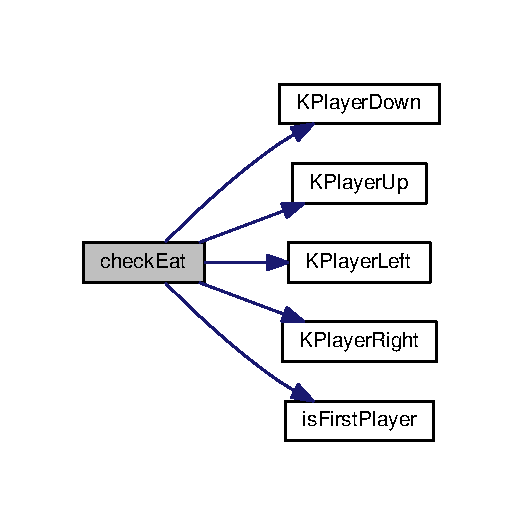
\includegraphics[width=251pt]{main_8cpp_aae35af58c079814bc6b5b300238173e0_cgraph}
\end{center}
\end{figure}




Here is the caller graph for this function\+:\nopagebreak
\begin{figure}[H]
\begin{center}
\leavevmode
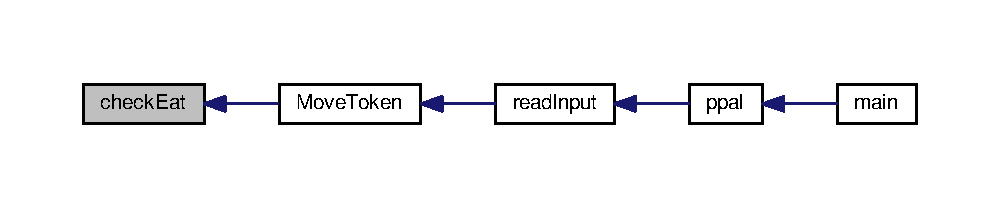
\includegraphics[width=350pt]{main_8cpp_aae35af58c079814bc6b5b300238173e0_icgraph}
\end{center}
\end{figure}


\index{main.\+cpp@{main.\+cpp}!Clear\+Screen@{Clear\+Screen}}
\index{Clear\+Screen@{Clear\+Screen}!main.\+cpp@{main.\+cpp}}
\subsubsection[{\texorpdfstring{Clear\+Screen()}{ClearScreen()}}]{\setlength{\rightskip}{0pt plus 5cm}void Clear\+Screen (
\begin{DoxyParamCaption}
{}
\end{DoxyParamCaption}
)}\hypertarget{main_8cpp_a6a3ca153f0817e8ba91a023b886bb662}{}\label{main_8cpp_a6a3ca153f0817e8ba91a023b886bb662}


Efface l\textquotesingle{}écran du terminal. 



Here is the call graph for this function\+:\nopagebreak
\begin{figure}[H]
\begin{center}
\leavevmode
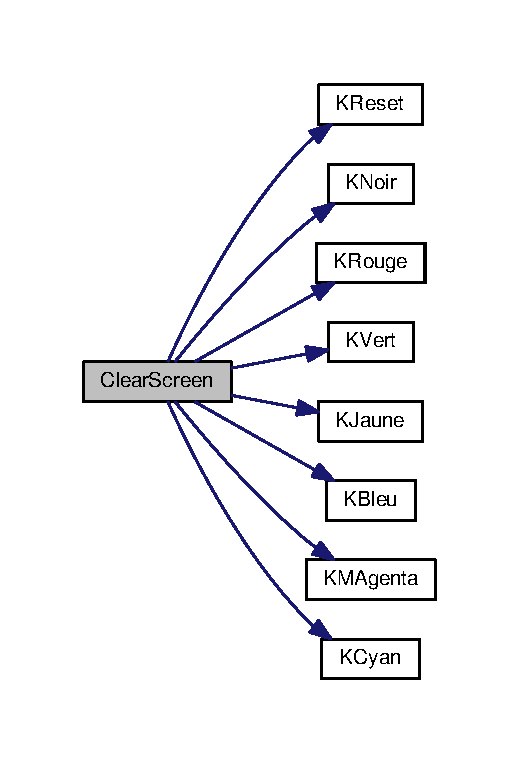
\includegraphics[width=249pt]{main_8cpp_a6a3ca153f0817e8ba91a023b886bb662_cgraph}
\end{center}
\end{figure}




Here is the caller graph for this function\+:\nopagebreak
\begin{figure}[H]
\begin{center}
\leavevmode
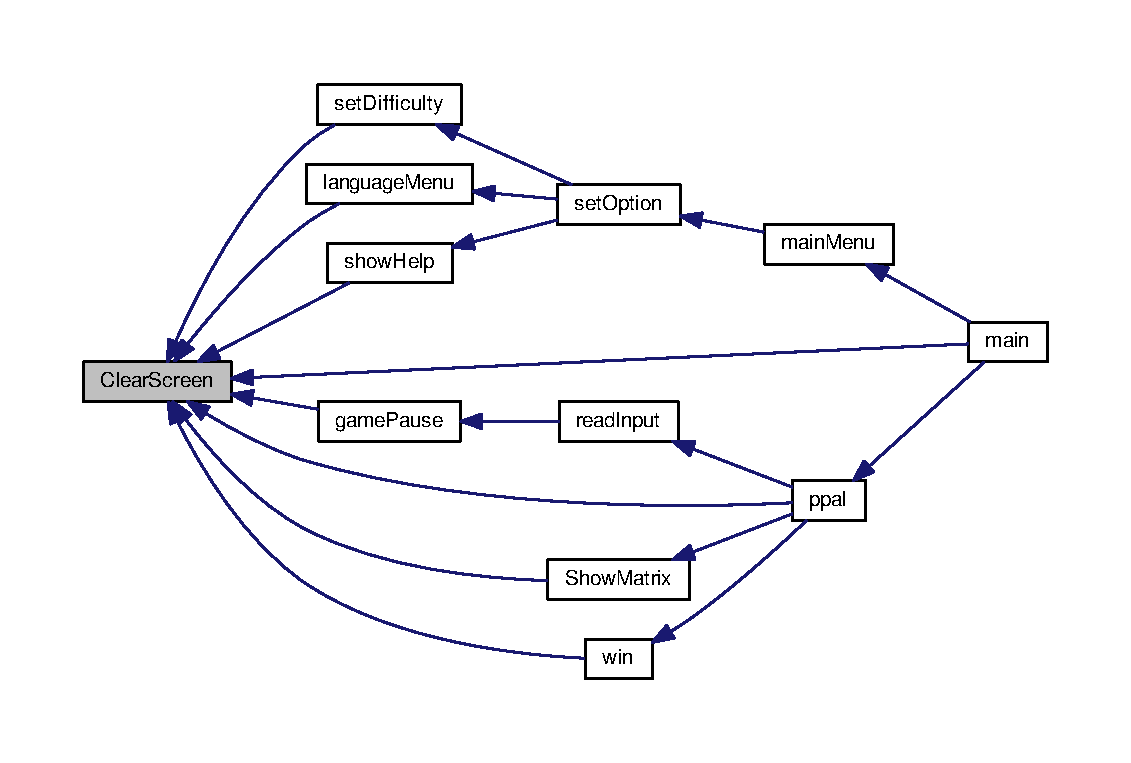
\includegraphics[width=350pt]{main_8cpp_a6a3ca153f0817e8ba91a023b886bb662_icgraph}
\end{center}
\end{figure}


\index{main.\+cpp@{main.\+cpp}!Couleur@{Couleur}}
\index{Couleur@{Couleur}!main.\+cpp@{main.\+cpp}}
\subsubsection[{\texorpdfstring{Couleur(const string \&coul)}{Couleur(const string &coul)}}]{\setlength{\rightskip}{0pt plus 5cm}void Couleur (
\begin{DoxyParamCaption}
\item[{const string \&}]{coul}
\end{DoxyParamCaption}
)}\hypertarget{main_8cpp_aa4699d640d199fc44a0c98dc6a5d45f5}{}\label{main_8cpp_aa4699d640d199fc44a0c98dc6a5d45f5}


Change la couleur des prochains caractères affichés. 


\begin{DoxyParams}[1]{Parameters}
\mbox{\tt in}  & {\em Code} & de la couleur à afficher \\
\hline
\end{DoxyParams}


Here is the caller graph for this function\+:\nopagebreak
\begin{figure}[H]
\begin{center}
\leavevmode
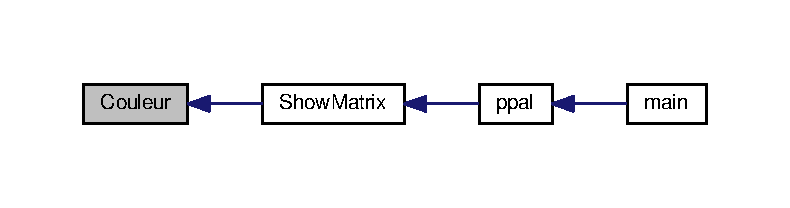
\includegraphics[width=350pt]{main_8cpp_aa4699d640d199fc44a0c98dc6a5d45f5_icgraph}
\end{center}
\end{figure}


\index{main.\+cpp@{main.\+cpp}!game\+Pause@{game\+Pause}}
\index{game\+Pause@{game\+Pause}!main.\+cpp@{main.\+cpp}}
\subsubsection[{\texorpdfstring{game\+Pause()}{gamePause()}}]{\setlength{\rightskip}{0pt plus 5cm}void game\+Pause (
\begin{DoxyParamCaption}
{}
\end{DoxyParamCaption}
)}\hypertarget{main_8cpp_aa5642769dce9d51ebe5be75b3dd5007e}{}\label{main_8cpp_aa5642769dce9d51ebe5be75b3dd5007e}


Met le jeu en pause. 



Here is the call graph for this function\+:\nopagebreak
\begin{figure}[H]
\begin{center}
\leavevmode
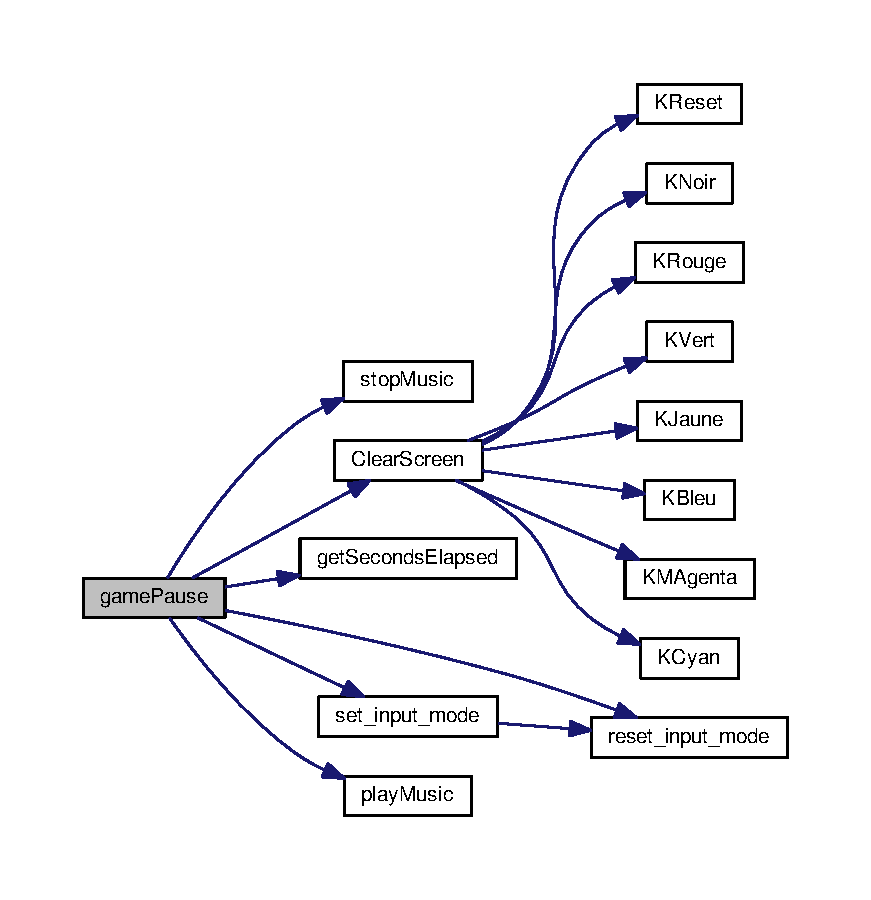
\includegraphics[width=350pt]{main_8cpp_aa5642769dce9d51ebe5be75b3dd5007e_cgraph}
\end{center}
\end{figure}




Here is the caller graph for this function\+:\nopagebreak
\begin{figure}[H]
\begin{center}
\leavevmode
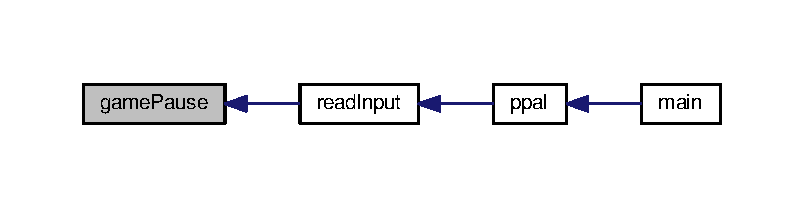
\includegraphics[width=350pt]{main_8cpp_aa5642769dce9d51ebe5be75b3dd5007e_icgraph}
\end{center}
\end{figure}


\index{main.\+cpp@{main.\+cpp}!get\+Color@{get\+Color}}
\index{get\+Color@{get\+Color}!main.\+cpp@{main.\+cpp}}
\subsubsection[{\texorpdfstring{get\+Color(string \&color)}{getColor(string &color)}}]{\setlength{\rightskip}{0pt plus 5cm}string get\+Color (
\begin{DoxyParamCaption}
\item[{string \&}]{color}
\end{DoxyParamCaption}
)}\hypertarget{main_8cpp_a669d365506d35e12f588d70c2c8c816b}{}\label{main_8cpp_a669d365506d35e12f588d70c2c8c816b}


Donne le code couleur d\textquotesingle{}une couleur. 


\begin{DoxyParams}{Parameters}
{\em La} & couleur recherchee \\
\hline
\end{DoxyParams}
\begin{DoxyReturn}{Returns}
Le code de la couleur donnee 
\end{DoxyReturn}


Here is the call graph for this function\+:\nopagebreak
\begin{figure}[H]
\begin{center}
\leavevmode
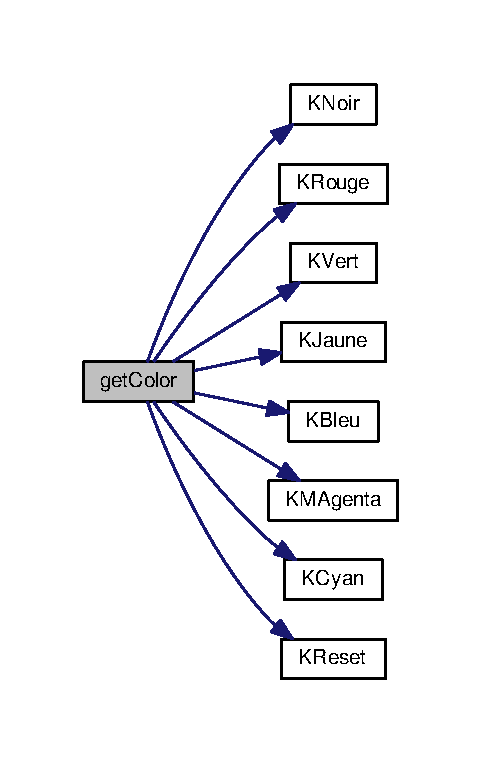
\includegraphics[width=231pt]{main_8cpp_a669d365506d35e12f588d70c2c8c816b_cgraph}
\end{center}
\end{figure}




Here is the caller graph for this function\+:\nopagebreak
\begin{figure}[H]
\begin{center}
\leavevmode
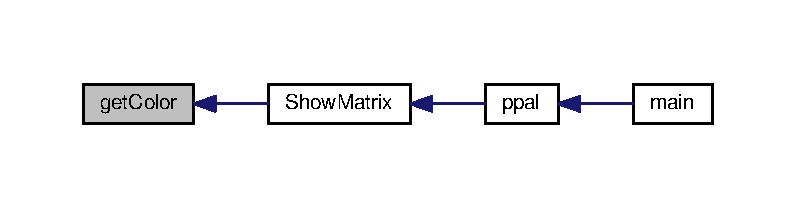
\includegraphics[width=350pt]{main_8cpp_a669d365506d35e12f588d70c2c8c816b_icgraph}
\end{center}
\end{figure}


\index{main.\+cpp@{main.\+cpp}!get\+Languages@{get\+Languages}}
\index{get\+Languages@{get\+Languages}!main.\+cpp@{main.\+cpp}}
\subsubsection[{\texorpdfstring{get\+Languages()}{getLanguages()}}]{\setlength{\rightskip}{0pt plus 5cm}vector$<$string$>$ get\+Languages (
\begin{DoxyParamCaption}
{}
\end{DoxyParamCaption}
)}\hypertarget{main_8cpp_a00b7c06ed44ae059cd27458c99605b8f}{}\label{main_8cpp_a00b7c06ed44ae059cd27458c99605b8f}


Fonction pour avoir la liste des langues disponibles. 

\begin{DoxyReturn}{Returns}
Un vecteur contenant les langues 
\end{DoxyReturn}


Here is the caller graph for this function\+:\nopagebreak
\begin{figure}[H]
\begin{center}
\leavevmode
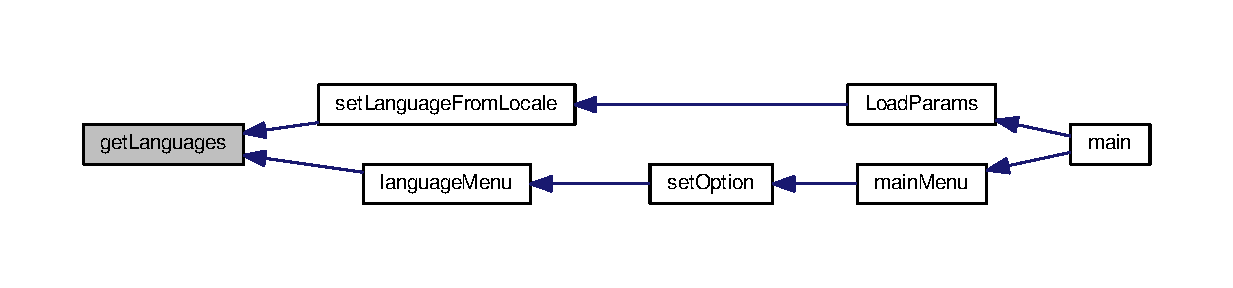
\includegraphics[width=350pt]{main_8cpp_a00b7c06ed44ae059cd27458c99605b8f_icgraph}
\end{center}
\end{figure}


\index{main.\+cpp@{main.\+cpp}!get\+Seconds\+Elapsed@{get\+Seconds\+Elapsed}}
\index{get\+Seconds\+Elapsed@{get\+Seconds\+Elapsed}!main.\+cpp@{main.\+cpp}}
\subsubsection[{\texorpdfstring{get\+Seconds\+Elapsed()}{getSecondsElapsed()}}]{\setlength{\rightskip}{0pt plus 5cm}unsigned get\+Seconds\+Elapsed (
\begin{DoxyParamCaption}
{}
\end{DoxyParamCaption}
)}\hypertarget{main_8cpp_a3c5e57d9be7dd4fad267101d26d1ab3c}{}\label{main_8cpp_a3c5e57d9be7dd4fad267101d26d1ab3c}


Donne le nombre de secondes ecoulées depuis le debut du chronometre. 

\begin{DoxyReturn}{Returns}
Le nombre de seconde ecoulees 
\end{DoxyReturn}


Here is the caller graph for this function\+:\nopagebreak
\begin{figure}[H]
\begin{center}
\leavevmode
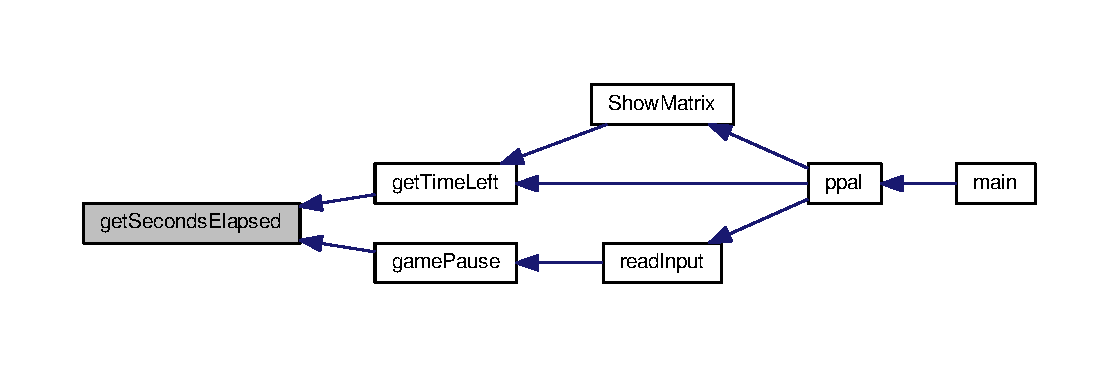
\includegraphics[width=350pt]{main_8cpp_a3c5e57d9be7dd4fad267101d26d1ab3c_icgraph}
\end{center}
\end{figure}


\index{main.\+cpp@{main.\+cpp}!get\+Time\+Left@{get\+Time\+Left}}
\index{get\+Time\+Left@{get\+Time\+Left}!main.\+cpp@{main.\+cpp}}
\subsubsection[{\texorpdfstring{get\+Time\+Left()}{getTimeLeft()}}]{\setlength{\rightskip}{0pt plus 5cm}int get\+Time\+Left (
\begin{DoxyParamCaption}
{}
\end{DoxyParamCaption}
)}\hypertarget{main_8cpp_a77241579fb9d12bcfefac569bde45fea}{}\label{main_8cpp_a77241579fb9d12bcfefac569bde45fea}


Donne le temps restant aux joueurs. 

\begin{DoxyReturn}{Returns}
Le temps restant 
\end{DoxyReturn}


Here is the call graph for this function\+:\nopagebreak
\begin{figure}[H]
\begin{center}
\leavevmode
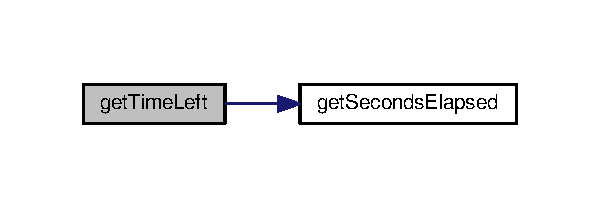
\includegraphics[width=288pt]{main_8cpp_a77241579fb9d12bcfefac569bde45fea_cgraph}
\end{center}
\end{figure}




Here is the caller graph for this function\+:\nopagebreak
\begin{figure}[H]
\begin{center}
\leavevmode
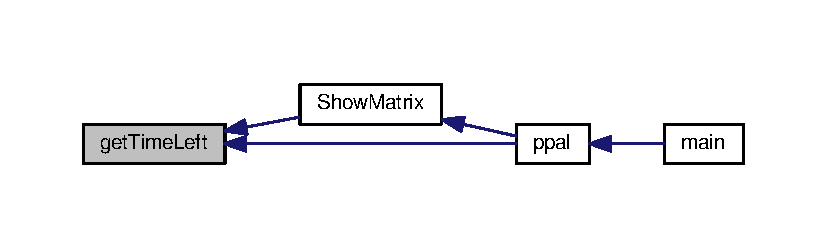
\includegraphics[width=350pt]{main_8cpp_a77241579fb9d12bcfefac569bde45fea_icgraph}
\end{center}
\end{figure}


\index{main.\+cpp@{main.\+cpp}!get\+Window\+Size@{get\+Window\+Size}}
\index{get\+Window\+Size@{get\+Window\+Size}!main.\+cpp@{main.\+cpp}}
\subsubsection[{\texorpdfstring{get\+Window\+Size(\+C\+Terminal\+Size \&\+Size)}{getWindowSize(CTerminalSize &Size)}}]{\setlength{\rightskip}{0pt plus 5cm}void get\+Window\+Size (
\begin{DoxyParamCaption}
\item[{{\bf C\+Terminal\+Size} \&}]{Size}
\end{DoxyParamCaption}
)}\hypertarget{main_8cpp_ac5311ed972004383e44c9e171a42642c}{}\label{main_8cpp_ac5311ed972004383e44c9e171a42642c}


Fonction pour avoir la taille de la fenetre. 


\begin{DoxyParams}{Parameters}
{\em La} & variable de taille \\
\hline
\end{DoxyParams}


Here is the caller graph for this function\+:\nopagebreak
\begin{figure}[H]
\begin{center}
\leavevmode
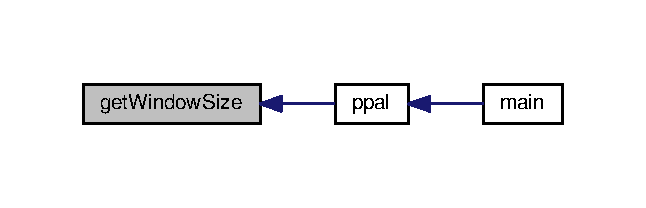
\includegraphics[width=310pt]{main_8cpp_ac5311ed972004383e44c9e171a42642c_icgraph}
\end{center}
\end{figure}


\index{main.\+cpp@{main.\+cpp}!Init\+Mat@{Init\+Mat}}
\index{Init\+Mat@{Init\+Mat}!main.\+cpp@{main.\+cpp}}
\subsubsection[{\texorpdfstring{Init\+Mat(\+C\+Matrix \&\+Mat, unsigned Nb\+Line, unsigned Nb\+Column, C\+Position \&\+Pos\+Player1, C\+Position \&\+Pos\+Player2)}{InitMat(CMatrix &Mat, unsigned NbLine, unsigned NbColumn, CPosition &PosPlayer1, CPosition &PosPlayer2)}}]{\setlength{\rightskip}{0pt plus 5cm}void Init\+Mat (
\begin{DoxyParamCaption}
\item[{{\bf C\+Matrix} \&}]{Mat, }
\item[{unsigned}]{Nb\+Line, }
\item[{unsigned}]{Nb\+Column, }
\item[{{\bf C\+Position} \&}]{Pos\+Player1, }
\item[{{\bf C\+Position} \&}]{Pos\+Player2}
\end{DoxyParamCaption}
)}\hypertarget{main_8cpp_a67a5b91aec2208cb14e67a4aa0659643}{}\label{main_8cpp_a67a5b91aec2208cb14e67a4aa0659643}


Initialise la grille de jeu. 


\begin{DoxyParams}{Parameters}
{\em La} & grille a initialiser \\
\hline
{\em Le} & nombre de lignes \\
\hline
{\em Le} & nombres de colonnes \\
\hline
{\em La} & position du joueur 1 \\
\hline
{\em La} & position du joueur 2 \\
\hline
\end{DoxyParams}


Here is the call graph for this function\+:\nopagebreak
\begin{figure}[H]
\begin{center}
\leavevmode
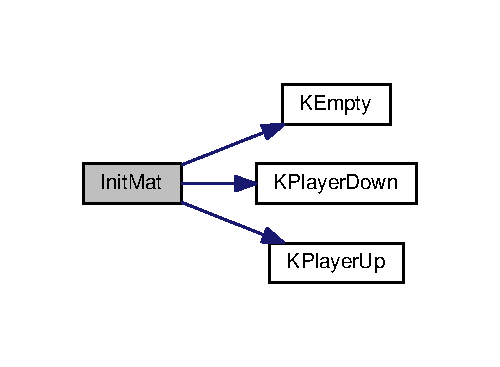
\includegraphics[width=240pt]{main_8cpp_a67a5b91aec2208cb14e67a4aa0659643_cgraph}
\end{center}
\end{figure}




Here is the caller graph for this function\+:\nopagebreak
\begin{figure}[H]
\begin{center}
\leavevmode
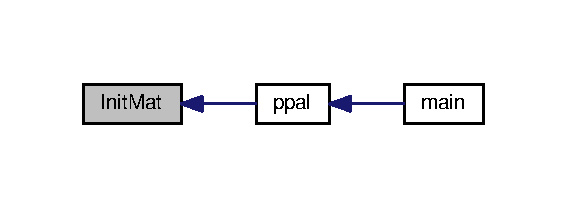
\includegraphics[width=272pt]{main_8cpp_a67a5b91aec2208cb14e67a4aa0659643_icgraph}
\end{center}
\end{figure}


\index{main.\+cpp@{main.\+cpp}!K\+Bleu@{K\+Bleu}}
\index{K\+Bleu@{K\+Bleu}!main.\+cpp@{main.\+cpp}}
\subsubsection[{\texorpdfstring{K\+Bleu(""34"")}{KBleu("34")}}]{\setlength{\rightskip}{0pt plus 5cm}const string K\+Bleu (
\begin{DoxyParamCaption}
\item[{\char`\"{}34\char`\"{}}]{}
\end{DoxyParamCaption}
)}\hypertarget{main_8cpp_a566a648bad2891bdf1d5746fed6fc6d3}{}\label{main_8cpp_a566a648bad2891bdf1d5746fed6fc6d3}


Code couleur bleu. 



Here is the caller graph for this function\+:\nopagebreak
\begin{figure}[H]
\begin{center}
\leavevmode
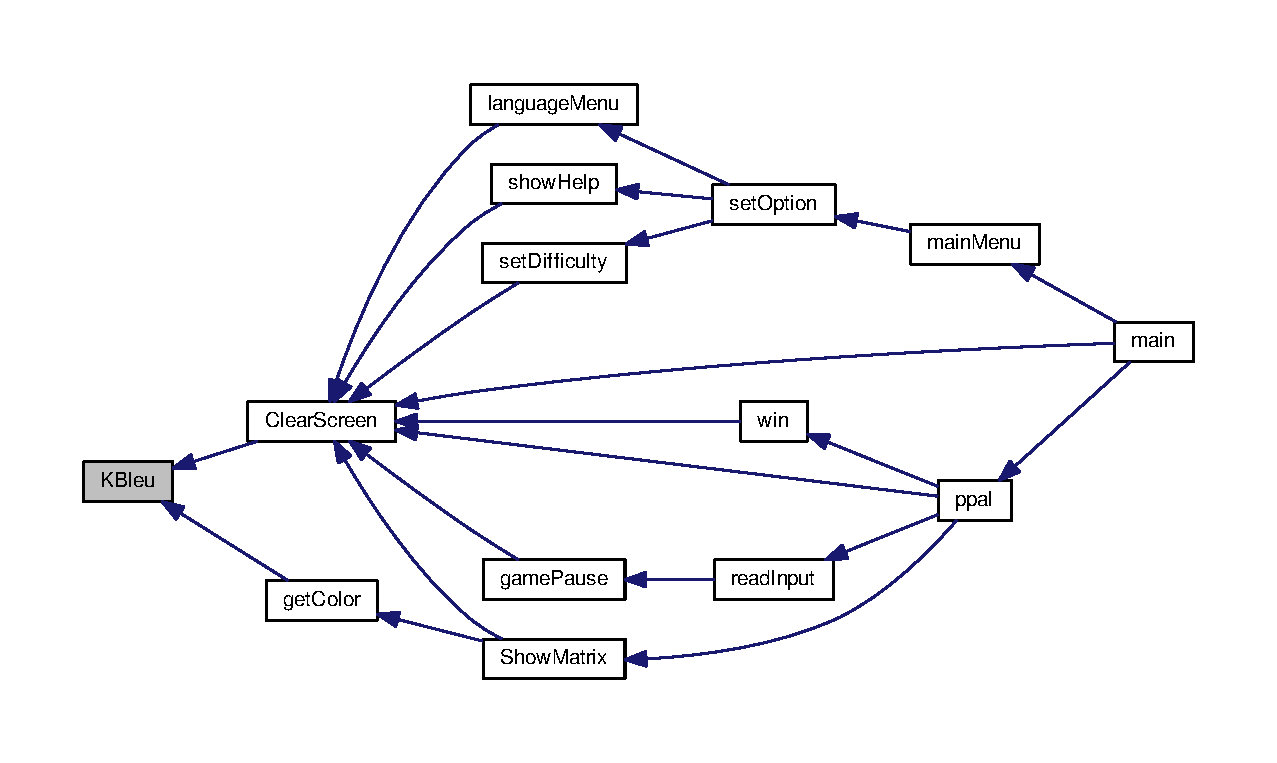
\includegraphics[width=350pt]{main_8cpp_a566a648bad2891bdf1d5746fed6fc6d3_icgraph}
\end{center}
\end{figure}


\index{main.\+cpp@{main.\+cpp}!K\+Cyan@{K\+Cyan}}
\index{K\+Cyan@{K\+Cyan}!main.\+cpp@{main.\+cpp}}
\subsubsection[{\texorpdfstring{K\+Cyan(""36"")}{KCyan("36")}}]{\setlength{\rightskip}{0pt plus 5cm}const string K\+Cyan (
\begin{DoxyParamCaption}
\item[{\char`\"{}36\char`\"{}}]{}
\end{DoxyParamCaption}
)}\hypertarget{main_8cpp_aa608863de5cd86b7b36f68a1189222cb}{}\label{main_8cpp_aa608863de5cd86b7b36f68a1189222cb}


Code couleur cyan. 



Here is the caller graph for this function\+:\nopagebreak
\begin{figure}[H]
\begin{center}
\leavevmode
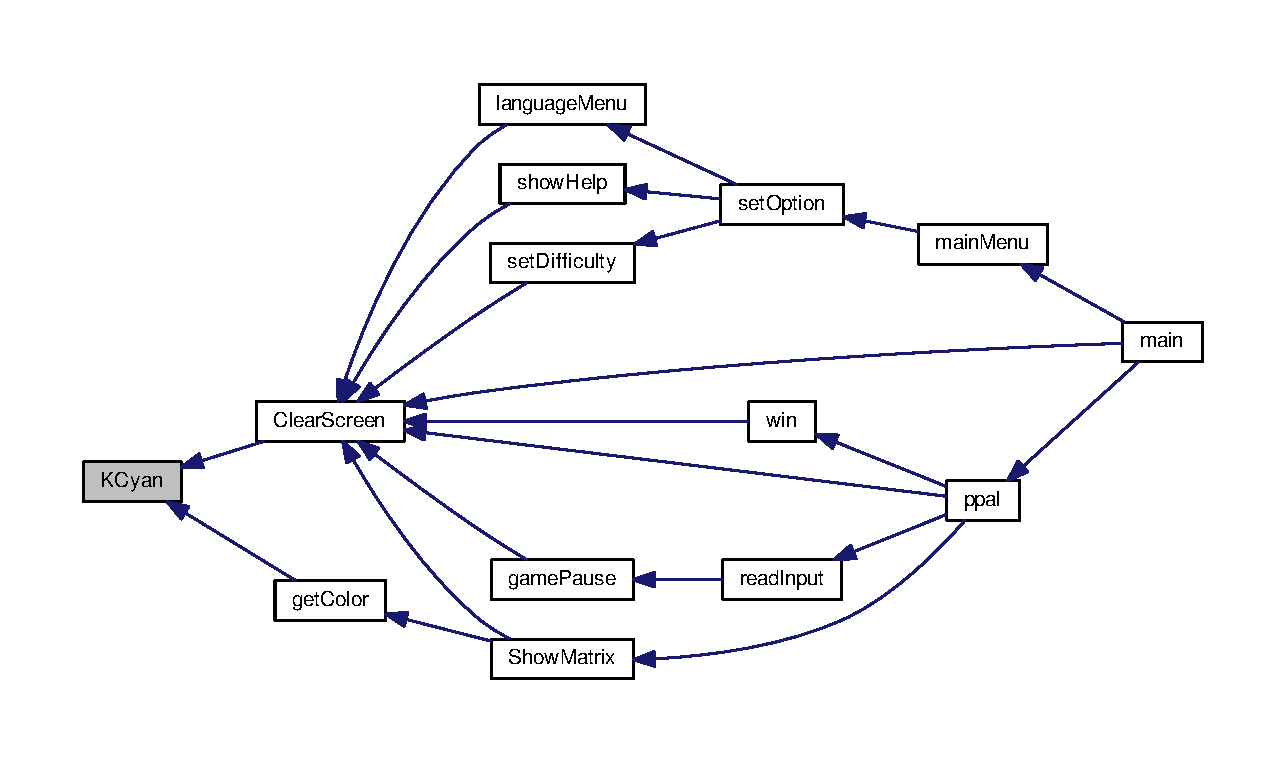
\includegraphics[width=350pt]{main_8cpp_aa608863de5cd86b7b36f68a1189222cb_icgraph}
\end{center}
\end{figure}


\index{main.\+cpp@{main.\+cpp}!K\+Empty@{K\+Empty}}
\index{K\+Empty@{K\+Empty}!main.\+cpp@{main.\+cpp}}
\subsubsection[{\texorpdfstring{K\+Empty(\textquotesingle{} \textquotesingle{})}{KEmpty(' ')}}]{\setlength{\rightskip}{0pt plus 5cm}const char K\+Empty (
\begin{DoxyParamCaption}
\item[{\textquotesingle{} \textquotesingle{}}]{}
\end{DoxyParamCaption}
)}\hypertarget{main_8cpp_a81a4a924185c81f623edfb38a4f629ed}{}\label{main_8cpp_a81a4a924185c81f623edfb38a4f629ed}


Espace vide. 



Here is the caller graph for this function\+:\nopagebreak
\begin{figure}[H]
\begin{center}
\leavevmode
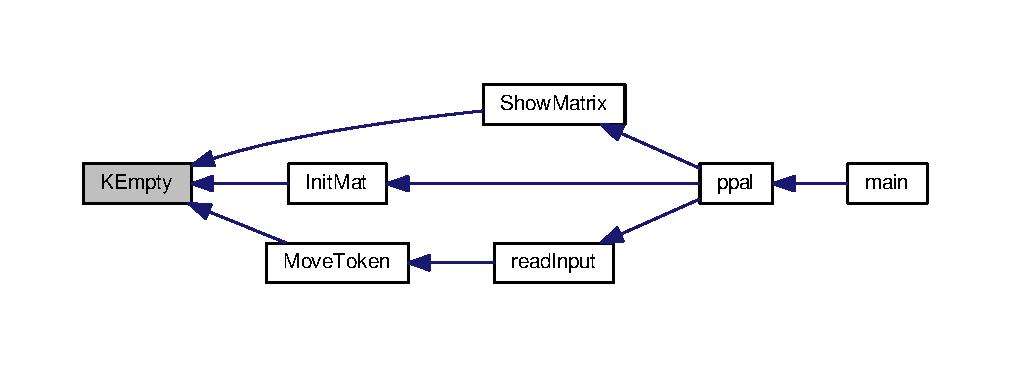
\includegraphics[width=350pt]{main_8cpp_a81a4a924185c81f623edfb38a4f629ed_icgraph}
\end{center}
\end{figure}


\index{main.\+cpp@{main.\+cpp}!K\+Jaune@{K\+Jaune}}
\index{K\+Jaune@{K\+Jaune}!main.\+cpp@{main.\+cpp}}
\subsubsection[{\texorpdfstring{K\+Jaune(""33"")}{KJaune("33")}}]{\setlength{\rightskip}{0pt plus 5cm}const string K\+Jaune (
\begin{DoxyParamCaption}
\item[{\char`\"{}33\char`\"{}}]{}
\end{DoxyParamCaption}
)}\hypertarget{main_8cpp_af02736496532ff1e9c9137691bfb1e07}{}\label{main_8cpp_af02736496532ff1e9c9137691bfb1e07}


Code couleur jaune. 



Here is the caller graph for this function\+:\nopagebreak
\begin{figure}[H]
\begin{center}
\leavevmode
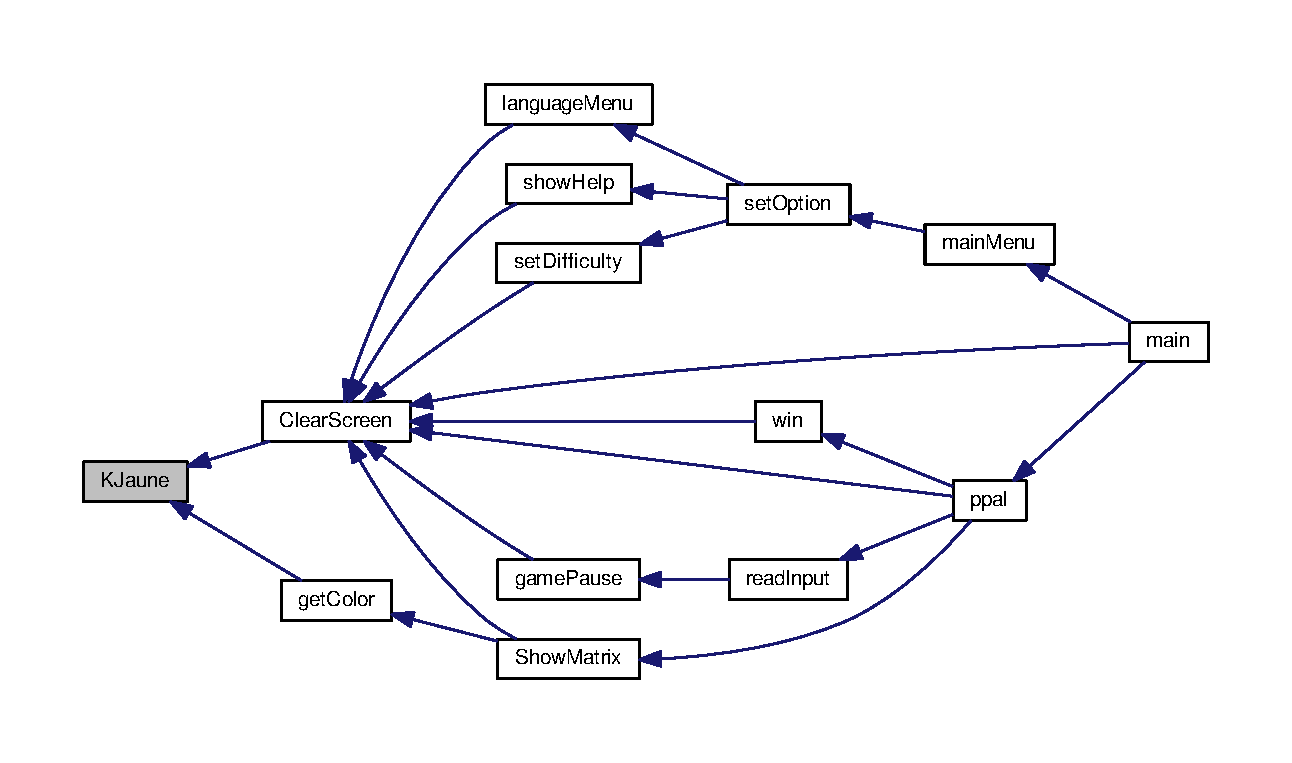
\includegraphics[width=350pt]{main_8cpp_af02736496532ff1e9c9137691bfb1e07_icgraph}
\end{center}
\end{figure}


\index{main.\+cpp@{main.\+cpp}!K\+M\+Agenta@{K\+M\+Agenta}}
\index{K\+M\+Agenta@{K\+M\+Agenta}!main.\+cpp@{main.\+cpp}}
\subsubsection[{\texorpdfstring{K\+M\+Agenta(""35"")}{KMAgenta("35")}}]{\setlength{\rightskip}{0pt plus 5cm}const string K\+M\+Agenta (
\begin{DoxyParamCaption}
\item[{\char`\"{}35\char`\"{}}]{}
\end{DoxyParamCaption}
)}\hypertarget{main_8cpp_a0eb078e8b0f7aa0c81169197965bbdd2}{}\label{main_8cpp_a0eb078e8b0f7aa0c81169197965bbdd2}


Code couleur magenta. 



Here is the caller graph for this function\+:\nopagebreak
\begin{figure}[H]
\begin{center}
\leavevmode
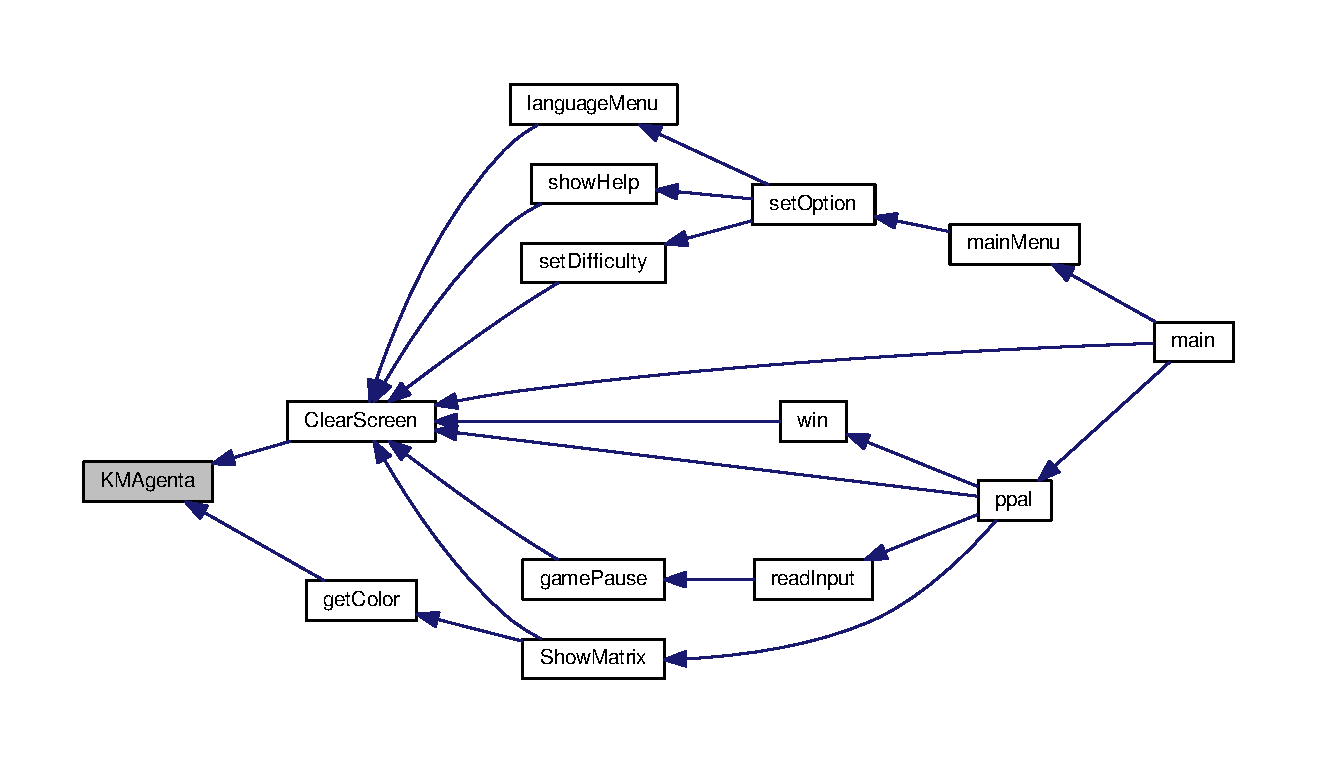
\includegraphics[width=350pt]{main_8cpp_a0eb078e8b0f7aa0c81169197965bbdd2_icgraph}
\end{center}
\end{figure}


\index{main.\+cpp@{main.\+cpp}!K\+Noir@{K\+Noir}}
\index{K\+Noir@{K\+Noir}!main.\+cpp@{main.\+cpp}}
\subsubsection[{\texorpdfstring{K\+Noir(""30"")}{KNoir("30")}}]{\setlength{\rightskip}{0pt plus 5cm}const string K\+Noir (
\begin{DoxyParamCaption}
\item[{\char`\"{}30\char`\"{}}]{}
\end{DoxyParamCaption}
)}\hypertarget{main_8cpp_a660c3e68e5967e553ae7fd9fb7073bbe}{}\label{main_8cpp_a660c3e68e5967e553ae7fd9fb7073bbe}


Code couleur noir. 



Here is the caller graph for this function\+:\nopagebreak
\begin{figure}[H]
\begin{center}
\leavevmode
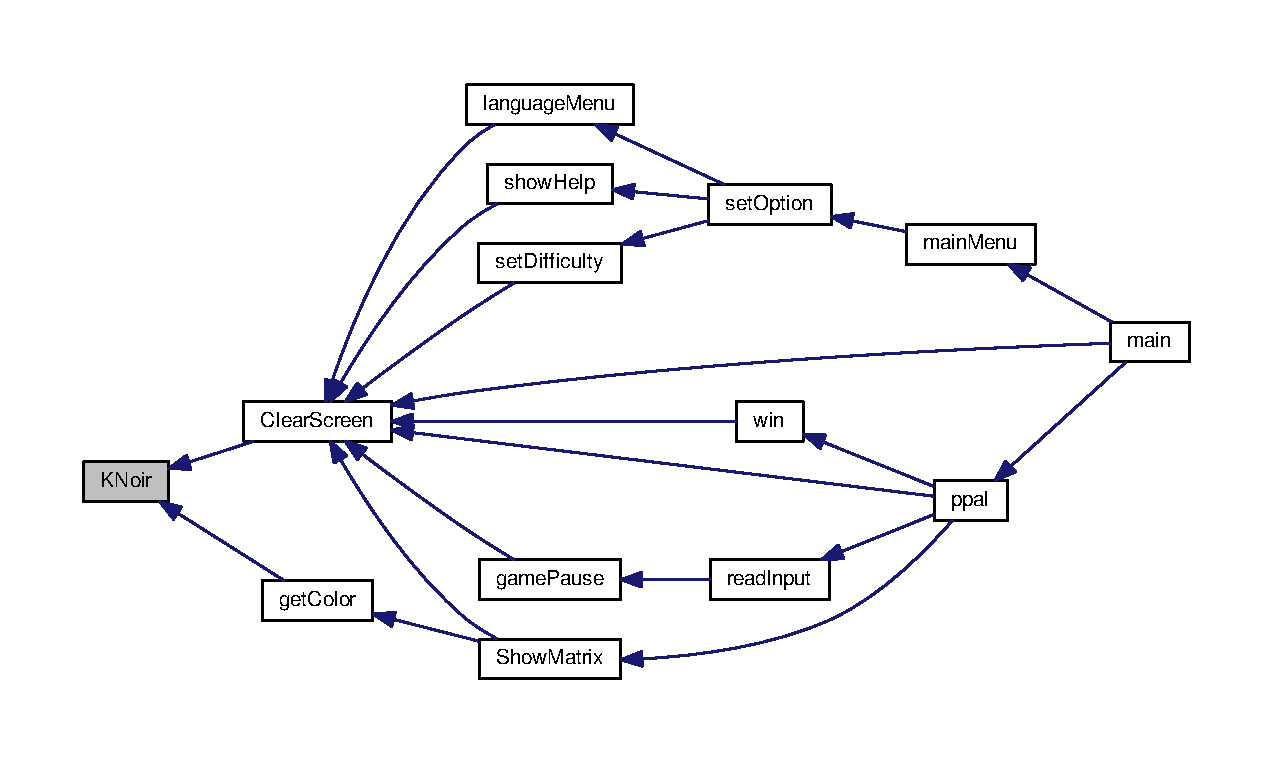
\includegraphics[width=350pt]{main_8cpp_a660c3e68e5967e553ae7fd9fb7073bbe_icgraph}
\end{center}
\end{figure}


\index{main.\+cpp@{main.\+cpp}!K\+Player\+Down@{K\+Player\+Down}}
\index{K\+Player\+Down@{K\+Player\+Down}!main.\+cpp@{main.\+cpp}}
\subsubsection[{\texorpdfstring{K\+Player\+Down(\textquotesingle{}v\textquotesingle{})}{KPlayerDown('v')}}]{\setlength{\rightskip}{0pt plus 5cm}const char K\+Player\+Down (
\begin{DoxyParamCaption}
\item[{\textquotesingle{}v\textquotesingle{}}]{}
\end{DoxyParamCaption}
)}\hypertarget{main_8cpp_a9e68aa6a6900f7f9567ca2f689ae0bdc}{}\label{main_8cpp_a9e68aa6a6900f7f9567ca2f689ae0bdc}


Joueur allant en bas. 



Here is the caller graph for this function\+:\nopagebreak
\begin{figure}[H]
\begin{center}
\leavevmode
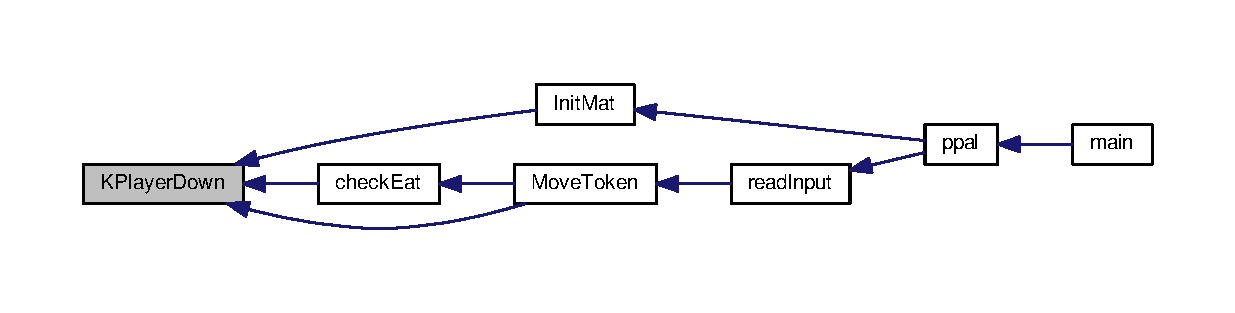
\includegraphics[width=350pt]{main_8cpp_a9e68aa6a6900f7f9567ca2f689ae0bdc_icgraph}
\end{center}
\end{figure}


\index{main.\+cpp@{main.\+cpp}!K\+Player\+Left@{K\+Player\+Left}}
\index{K\+Player\+Left@{K\+Player\+Left}!main.\+cpp@{main.\+cpp}}
\subsubsection[{\texorpdfstring{K\+Player\+Left(\textquotesingle{}$<$\textquotesingle{})}{KPlayerLeft('<')}}]{\setlength{\rightskip}{0pt plus 5cm}const char K\+Player\+Left (
\begin{DoxyParamCaption}
{}
\end{DoxyParamCaption}
)}\hypertarget{main_8cpp_a0e0be1c05bbe1c9a11c01d5b8b558a70}{}\label{main_8cpp_a0e0be1c05bbe1c9a11c01d5b8b558a70}


Joueur allant a gauche. 



Here is the caller graph for this function\+:\nopagebreak
\begin{figure}[H]
\begin{center}
\leavevmode
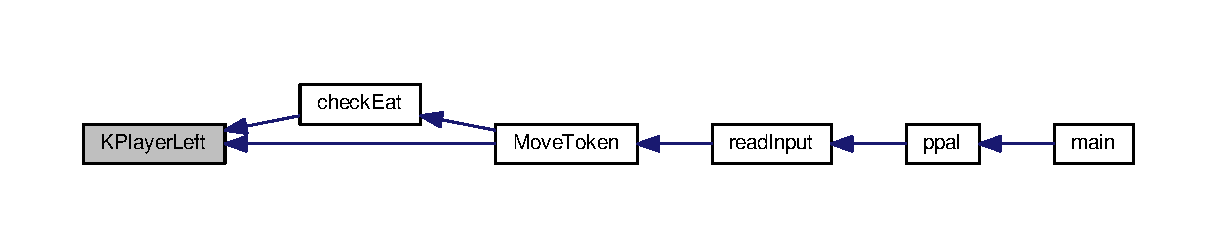
\includegraphics[width=350pt]{main_8cpp_a0e0be1c05bbe1c9a11c01d5b8b558a70_icgraph}
\end{center}
\end{figure}


\index{main.\+cpp@{main.\+cpp}!K\+Player\+Right@{K\+Player\+Right}}
\index{K\+Player\+Right@{K\+Player\+Right}!main.\+cpp@{main.\+cpp}}
\subsubsection[{\texorpdfstring{K\+Player\+Right(\textquotesingle{}$>$\textquotesingle{})}{KPlayerRight('>')}}]{\setlength{\rightskip}{0pt plus 5cm}const char K\+Player\+Right (
\begin{DoxyParamCaption}
\item[{\textquotesingle{}}]{, }
\item[{\textquotesingle{}}]{}
\end{DoxyParamCaption}
)}\hypertarget{main_8cpp_acedb4c0046e67a1ce8618258be548e07}{}\label{main_8cpp_acedb4c0046e67a1ce8618258be548e07}


Joueur allant à droite. 



Here is the caller graph for this function\+:\nopagebreak
\begin{figure}[H]
\begin{center}
\leavevmode
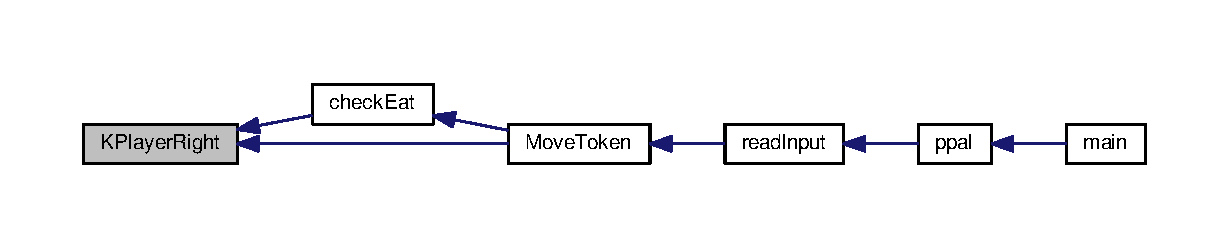
\includegraphics[width=350pt]{main_8cpp_acedb4c0046e67a1ce8618258be548e07_icgraph}
\end{center}
\end{figure}


\index{main.\+cpp@{main.\+cpp}!K\+Player\+Up@{K\+Player\+Up}}
\index{K\+Player\+Up@{K\+Player\+Up}!main.\+cpp@{main.\+cpp}}
\subsubsection[{\texorpdfstring{K\+Player\+Up(\textquotesingle{}$^\wedge$\textquotesingle{})}{KPlayerUp('^')}}]{\setlength{\rightskip}{0pt plus 5cm}const char K\+Player\+Up (
\begin{DoxyParamCaption}
\item[{\textquotesingle{}$^\wedge$\textquotesingle{}}]{}
\end{DoxyParamCaption}
)}\hypertarget{main_8cpp_a24d8d97414c569e372f4ff5c0a7e2fa0}{}\label{main_8cpp_a24d8d97414c569e372f4ff5c0a7e2fa0}


Joueur allant en haut. 



Here is the caller graph for this function\+:\nopagebreak
\begin{figure}[H]
\begin{center}
\leavevmode
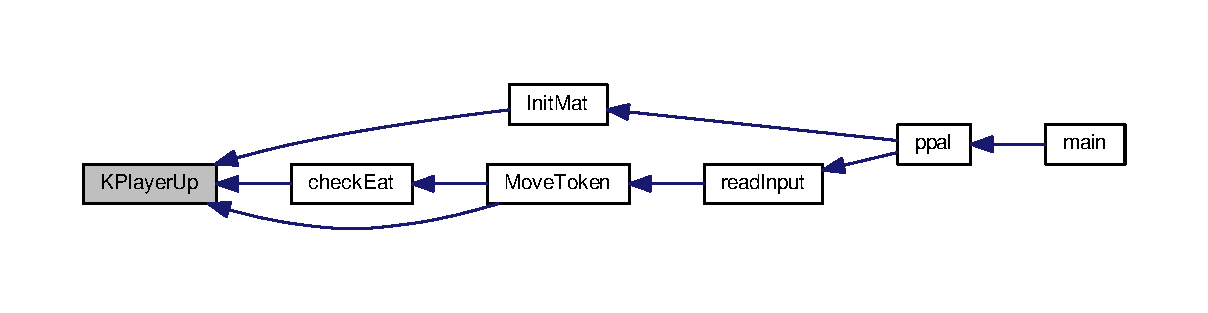
\includegraphics[width=350pt]{main_8cpp_a24d8d97414c569e372f4ff5c0a7e2fa0_icgraph}
\end{center}
\end{figure}


\index{main.\+cpp@{main.\+cpp}!K\+Reset@{K\+Reset}}
\index{K\+Reset@{K\+Reset}!main.\+cpp@{main.\+cpp}}
\subsubsection[{\texorpdfstring{K\+Reset(""0"")}{KReset("0")}}]{\setlength{\rightskip}{0pt plus 5cm}const string K\+Reset (
\begin{DoxyParamCaption}
\item[{\char`\"{}0\char`\"{}}]{}
\end{DoxyParamCaption}
)}\hypertarget{main_8cpp_ae421976620c052c8350660039b8cb3bd}{}\label{main_8cpp_ae421976620c052c8350660039b8cb3bd}


Code couleur nul (reinitialisation) 



Here is the caller graph for this function\+:\nopagebreak
\begin{figure}[H]
\begin{center}
\leavevmode
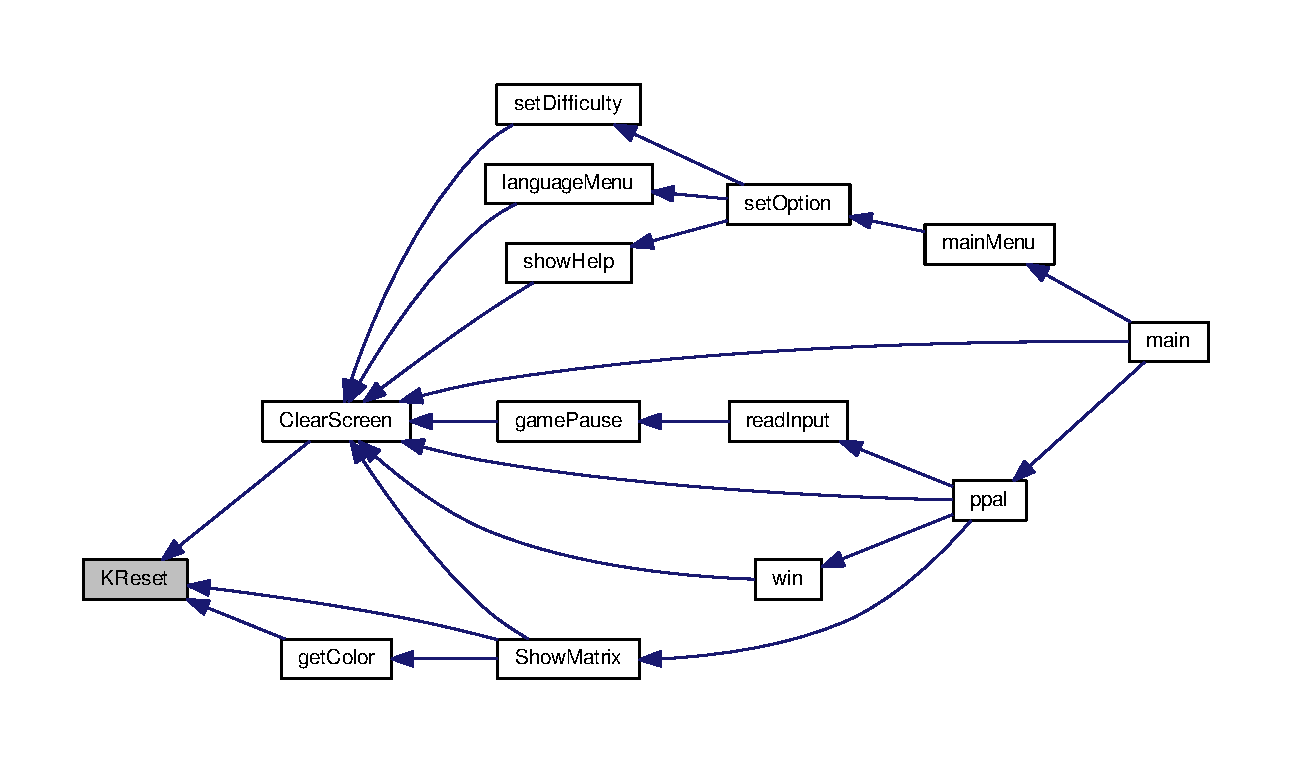
\includegraphics[width=350pt]{main_8cpp_ae421976620c052c8350660039b8cb3bd_icgraph}
\end{center}
\end{figure}


\index{main.\+cpp@{main.\+cpp}!K\+Rouge@{K\+Rouge}}
\index{K\+Rouge@{K\+Rouge}!main.\+cpp@{main.\+cpp}}
\subsubsection[{\texorpdfstring{K\+Rouge(""31"")}{KRouge("31")}}]{\setlength{\rightskip}{0pt plus 5cm}const string K\+Rouge (
\begin{DoxyParamCaption}
\item[{\char`\"{}31\char`\"{}}]{}
\end{DoxyParamCaption}
)}\hypertarget{main_8cpp_a09f08ffca2080e9ca9c050093a2ca6d5}{}\label{main_8cpp_a09f08ffca2080e9ca9c050093a2ca6d5}


Code couleur rouge. 



Here is the caller graph for this function\+:\nopagebreak
\begin{figure}[H]
\begin{center}
\leavevmode
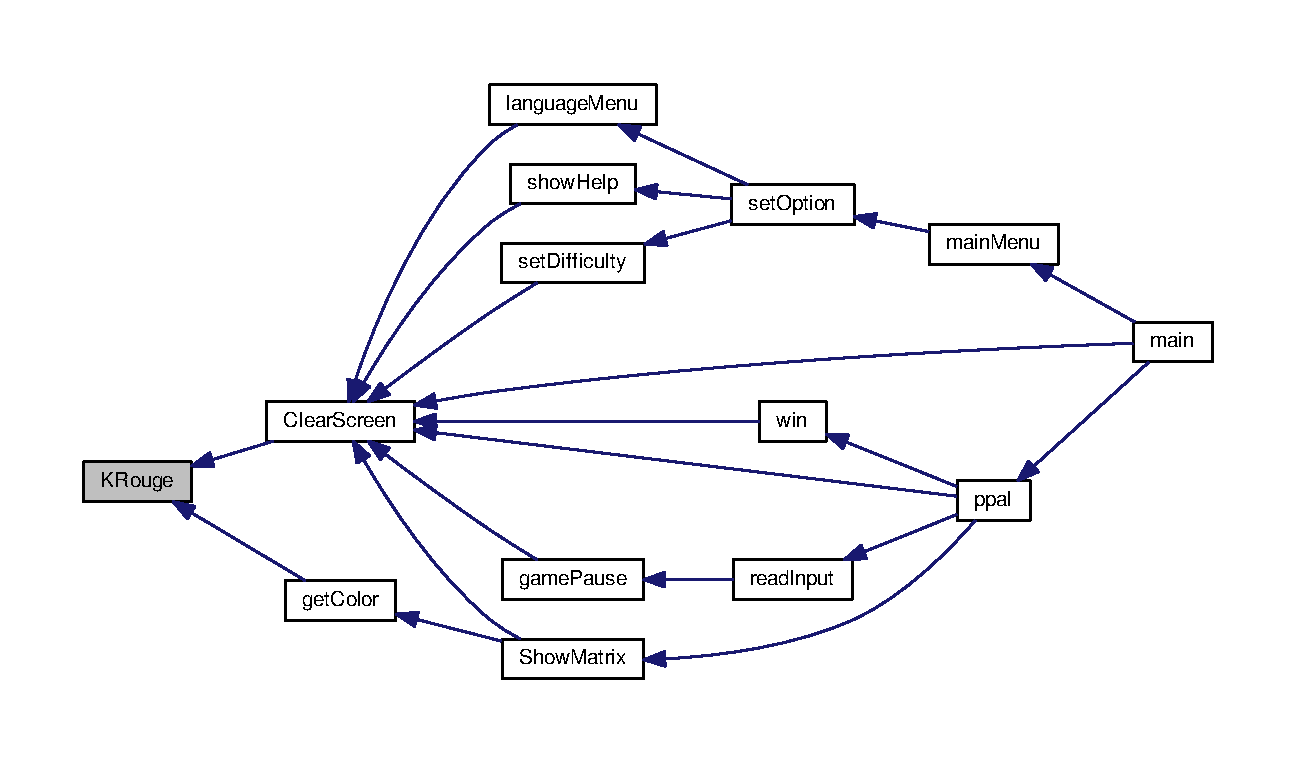
\includegraphics[width=350pt]{main_8cpp_a09f08ffca2080e9ca9c050093a2ca6d5_icgraph}
\end{center}
\end{figure}


\index{main.\+cpp@{main.\+cpp}!K\+Vert@{K\+Vert}}
\index{K\+Vert@{K\+Vert}!main.\+cpp@{main.\+cpp}}
\subsubsection[{\texorpdfstring{K\+Vert(""32"")}{KVert("32")}}]{\setlength{\rightskip}{0pt plus 5cm}const string K\+Vert (
\begin{DoxyParamCaption}
\item[{\char`\"{}32\char`\"{}}]{}
\end{DoxyParamCaption}
)}\hypertarget{main_8cpp_a1cdcc3e3fe7660a6f85532bb0d228fee}{}\label{main_8cpp_a1cdcc3e3fe7660a6f85532bb0d228fee}


Code couleur vert. 



Here is the caller graph for this function\+:\nopagebreak
\begin{figure}[H]
\begin{center}
\leavevmode
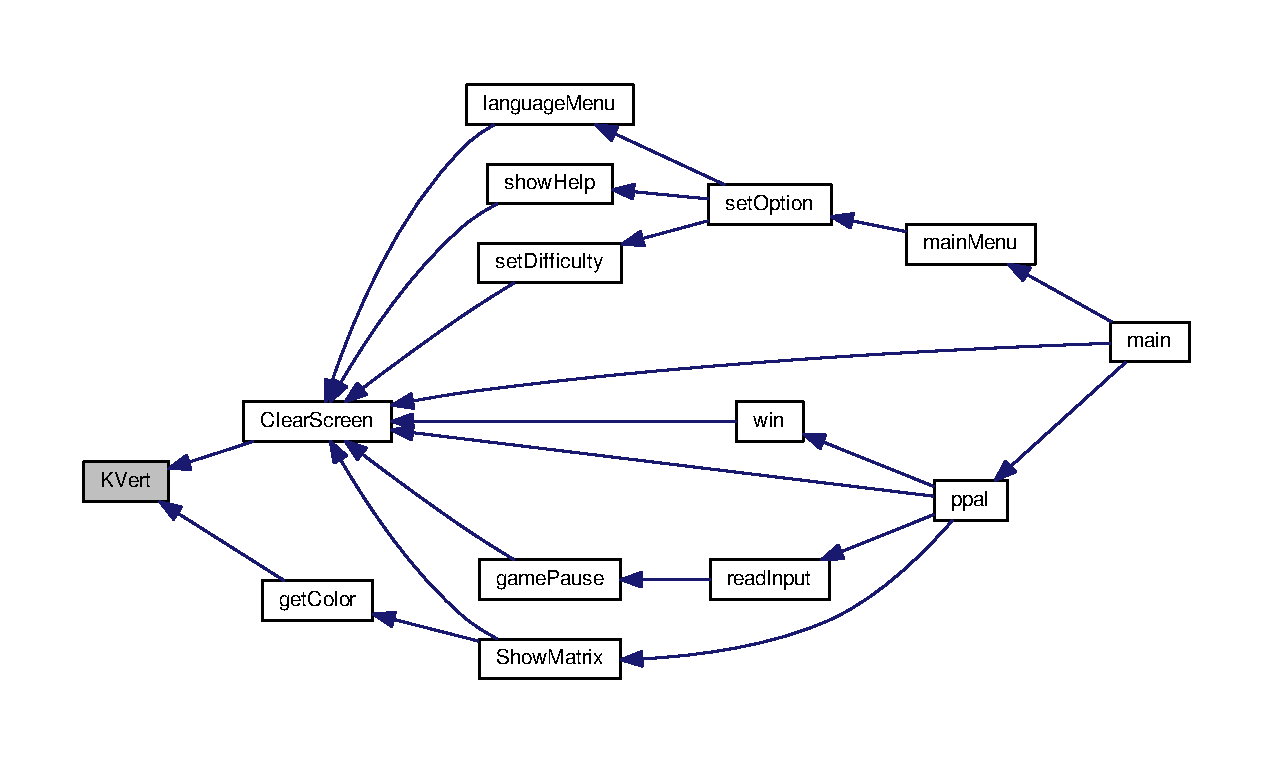
\includegraphics[width=350pt]{main_8cpp_a1cdcc3e3fe7660a6f85532bb0d228fee_icgraph}
\end{center}
\end{figure}


\index{main.\+cpp@{main.\+cpp}!language\+Menu@{language\+Menu}}
\index{language\+Menu@{language\+Menu}!main.\+cpp@{main.\+cpp}}
\subsubsection[{\texorpdfstring{language\+Menu()}{languageMenu()}}]{\setlength{\rightskip}{0pt plus 5cm}void language\+Menu (
\begin{DoxyParamCaption}
{}
\end{DoxyParamCaption}
)}\hypertarget{main_8cpp_a3b00a9c78e94cf30a9961b377729622c}{}\label{main_8cpp_a3b00a9c78e94cf30a9961b377729622c}


Affiche le menu de selection de la langue. 



Here is the call graph for this function\+:\nopagebreak
\begin{figure}[H]
\begin{center}
\leavevmode
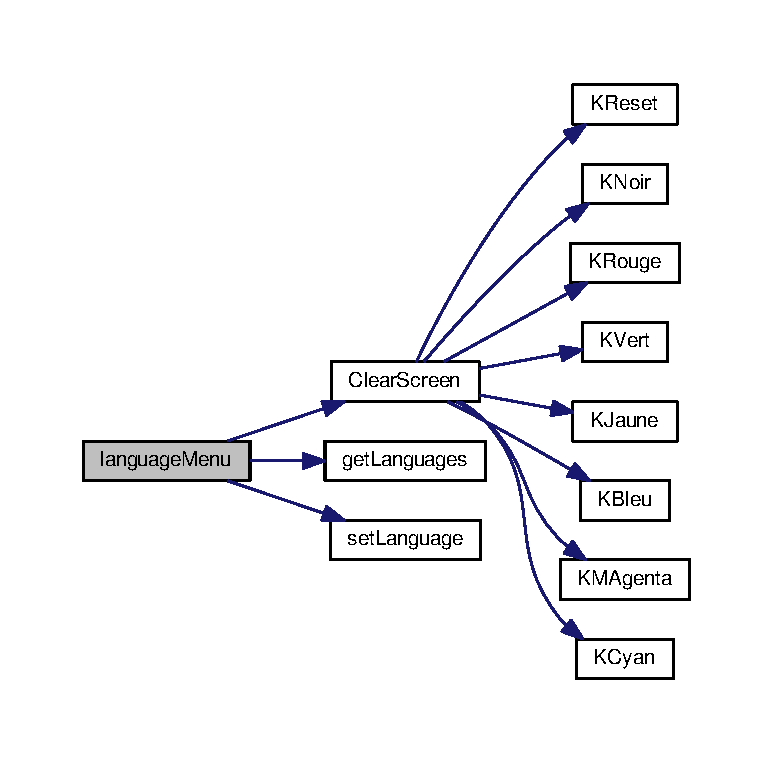
\includegraphics[width=350pt]{main_8cpp_a3b00a9c78e94cf30a9961b377729622c_cgraph}
\end{center}
\end{figure}




Here is the caller graph for this function\+:\nopagebreak
\begin{figure}[H]
\begin{center}
\leavevmode
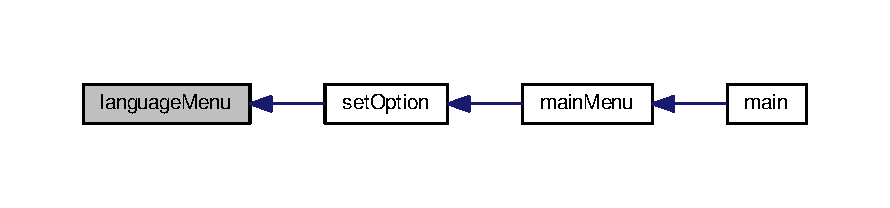
\includegraphics[width=350pt]{main_8cpp_a3b00a9c78e94cf30a9961b377729622c_icgraph}
\end{center}
\end{figure}


\index{main.\+cpp@{main.\+cpp}!Load\+Params@{Load\+Params}}
\index{Load\+Params@{Load\+Params}!main.\+cpp@{main.\+cpp}}
\subsubsection[{\texorpdfstring{Load\+Params(\+C\+My\+Param \&\+My\+Params)}{LoadParams(CMyParam &MyParams)}}]{\setlength{\rightskip}{0pt plus 5cm}void Load\+Params (
\begin{DoxyParamCaption}
\item[{{\bf C\+My\+Param} \&}]{My\+Params}
\end{DoxyParamCaption}
)}\hypertarget{main_8cpp_af700f5ec6a814c6f4dee71b71c54869e}{}\label{main_8cpp_af700f5ec6a814c6f4dee71b71c54869e}


Charge les parametres du jeu a partir du fichier config.\+yml. 


\begin{DoxyParams}{Parameters}
{\em Parametres} & du jeu \\
\hline
\end{DoxyParams}


Here is the call graph for this function\+:\nopagebreak
\begin{figure}[H]
\begin{center}
\leavevmode
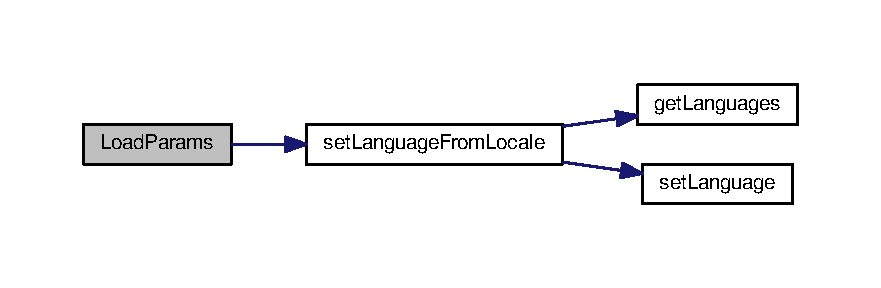
\includegraphics[width=350pt]{main_8cpp_af700f5ec6a814c6f4dee71b71c54869e_cgraph}
\end{center}
\end{figure}




Here is the caller graph for this function\+:\nopagebreak
\begin{figure}[H]
\begin{center}
\leavevmode
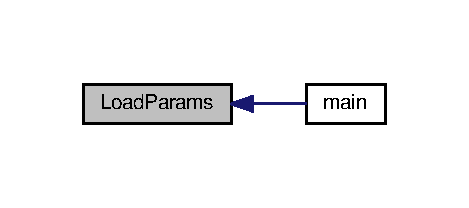
\includegraphics[width=225pt]{main_8cpp_af700f5ec6a814c6f4dee71b71c54869e_icgraph}
\end{center}
\end{figure}


\index{main.\+cpp@{main.\+cpp}!main@{main}}
\index{main@{main}!main.\+cpp@{main.\+cpp}}
\subsubsection[{\texorpdfstring{main()}{main()}}]{\setlength{\rightskip}{0pt plus 5cm}int main (
\begin{DoxyParamCaption}
{}
\end{DoxyParamCaption}
)}\hypertarget{main_8cpp_ae66f6b31b5ad750f1fe042a706a4e3d4}{}\label{main_8cpp_ae66f6b31b5ad750f1fe042a706a4e3d4}


Fonction principale. 

\begin{DoxyReturn}{Returns}
Le code de sortie du programme 
\end{DoxyReturn}


Here is the call graph for this function\+:
\nopagebreak
\begin{figure}[H]
\begin{center}
\leavevmode
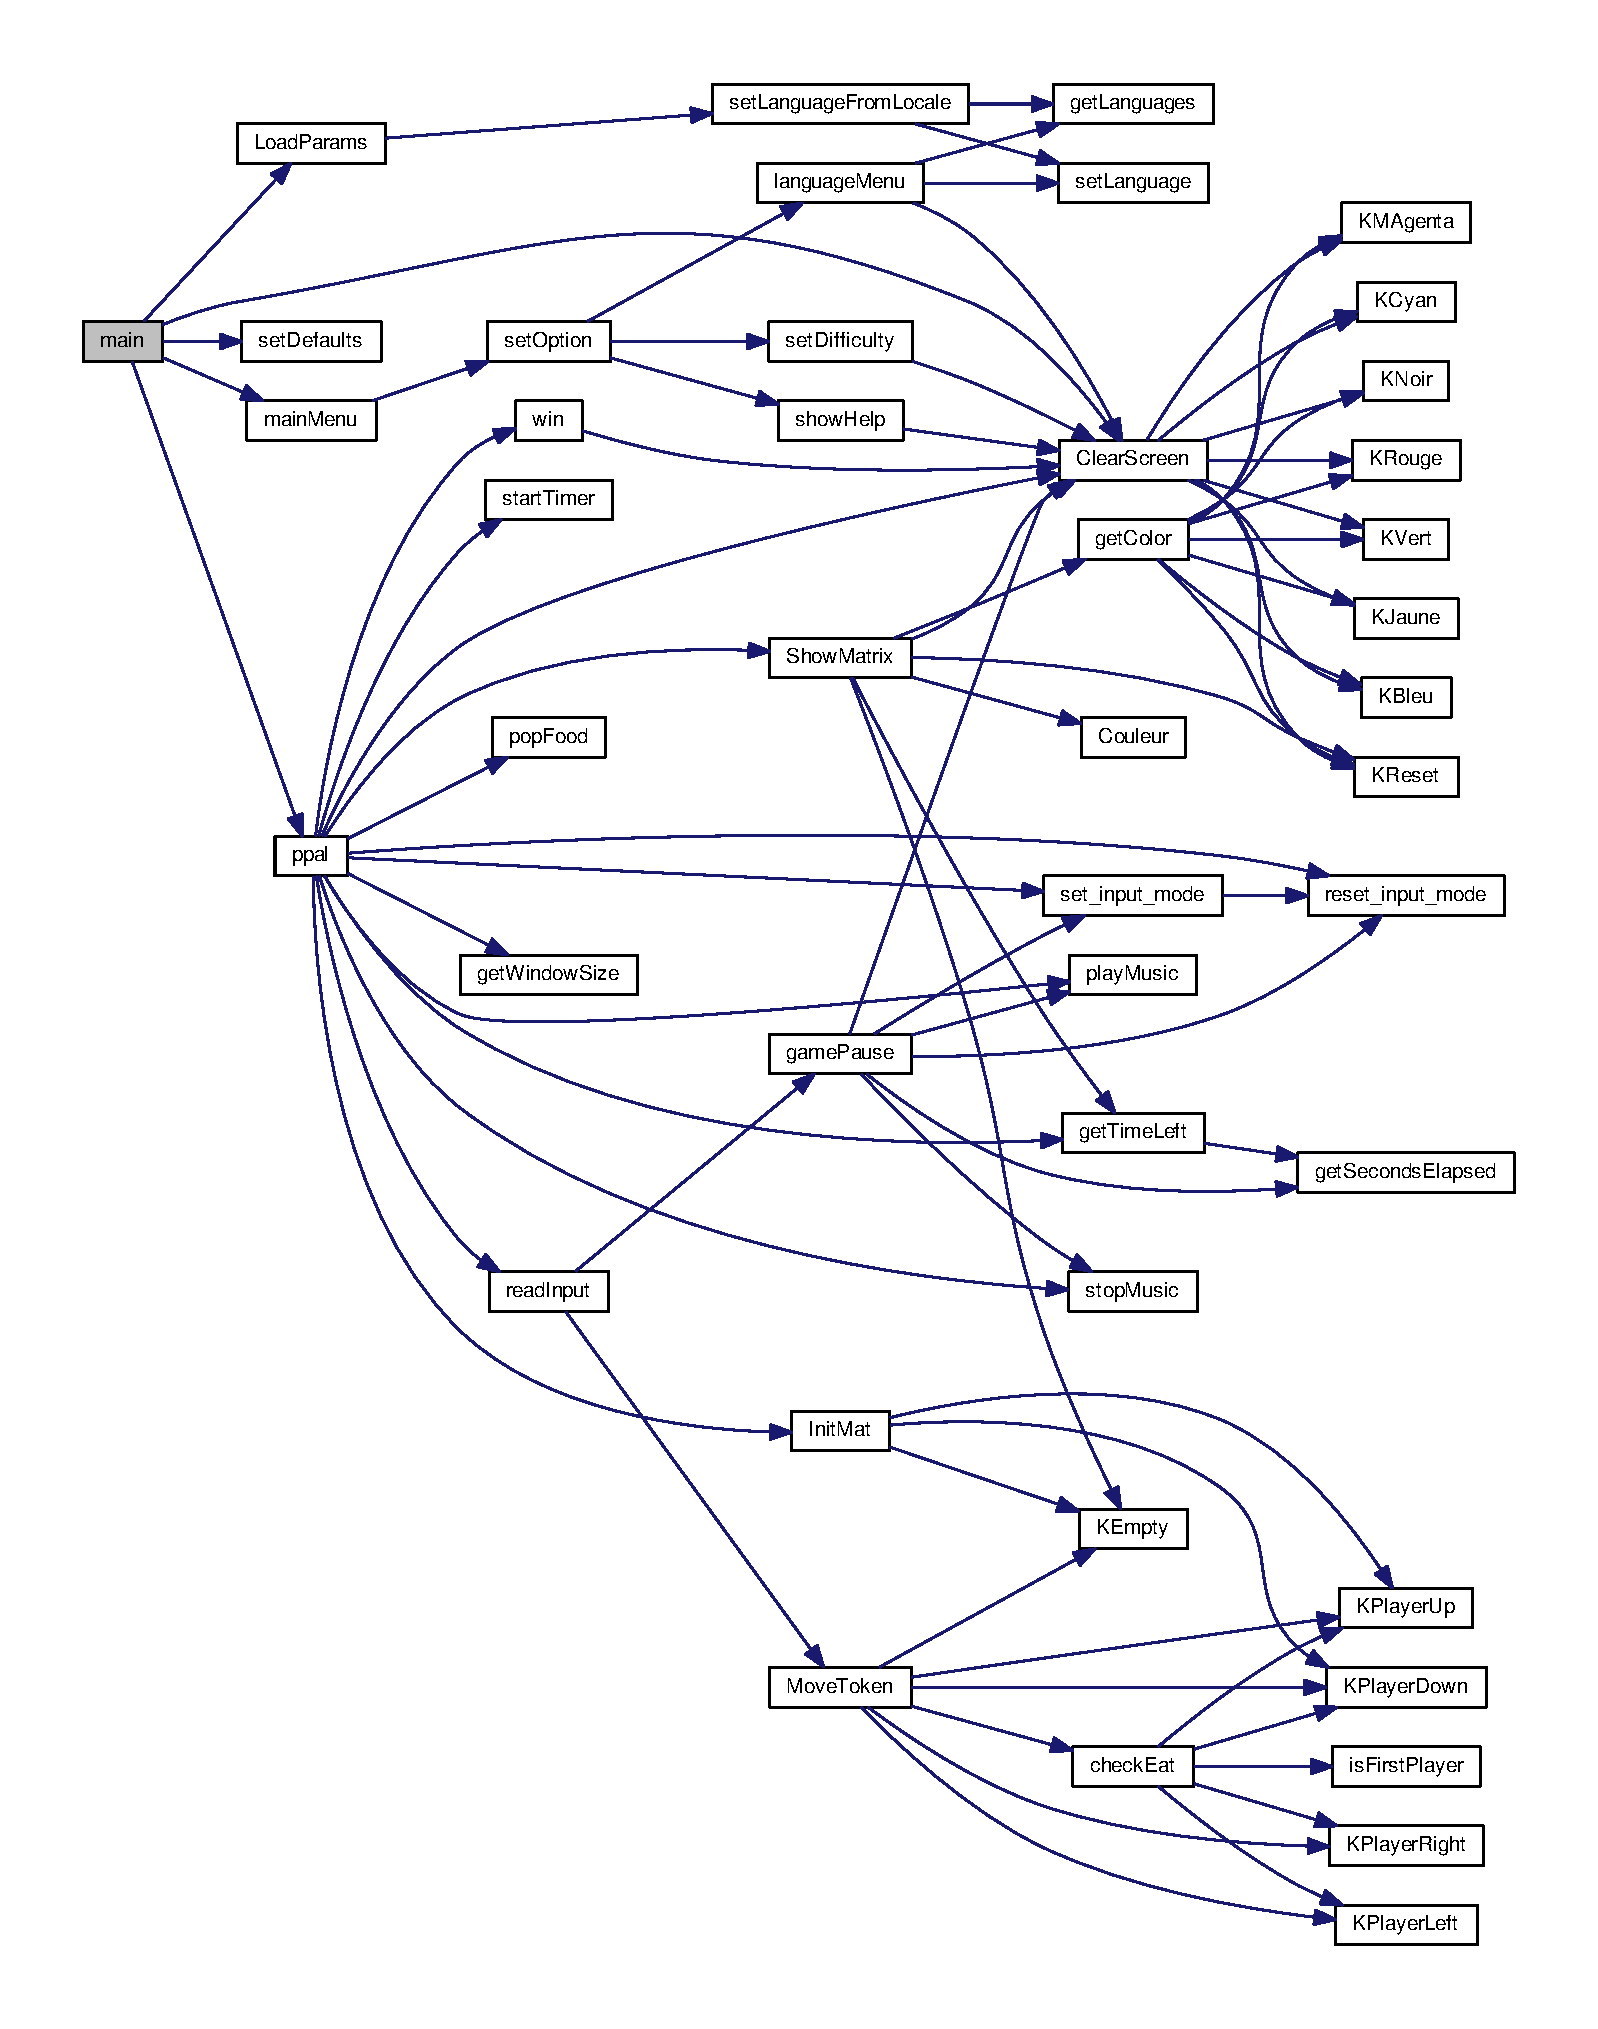
\includegraphics[width=350pt]{main_8cpp_ae66f6b31b5ad750f1fe042a706a4e3d4_cgraph}
\end{center}
\end{figure}


\index{main.\+cpp@{main.\+cpp}!main\+Menu@{main\+Menu}}
\index{main\+Menu@{main\+Menu}!main.\+cpp@{main.\+cpp}}
\subsubsection[{\texorpdfstring{main\+Menu()}{mainMenu()}}]{\setlength{\rightskip}{0pt plus 5cm}bool main\+Menu (
\begin{DoxyParamCaption}
{}
\end{DoxyParamCaption}
)}\hypertarget{main_8cpp_aaed5cc5349863a6b8a7a86c74f28263a}{}\label{main_8cpp_aaed5cc5349863a6b8a7a86c74f28263a}


Affiche le menu principal. 

\begin{DoxyReturn}{Returns}
Si le joueur veut jouer ou non 
\end{DoxyReturn}


Here is the call graph for this function\+:\nopagebreak
\begin{figure}[H]
\begin{center}
\leavevmode
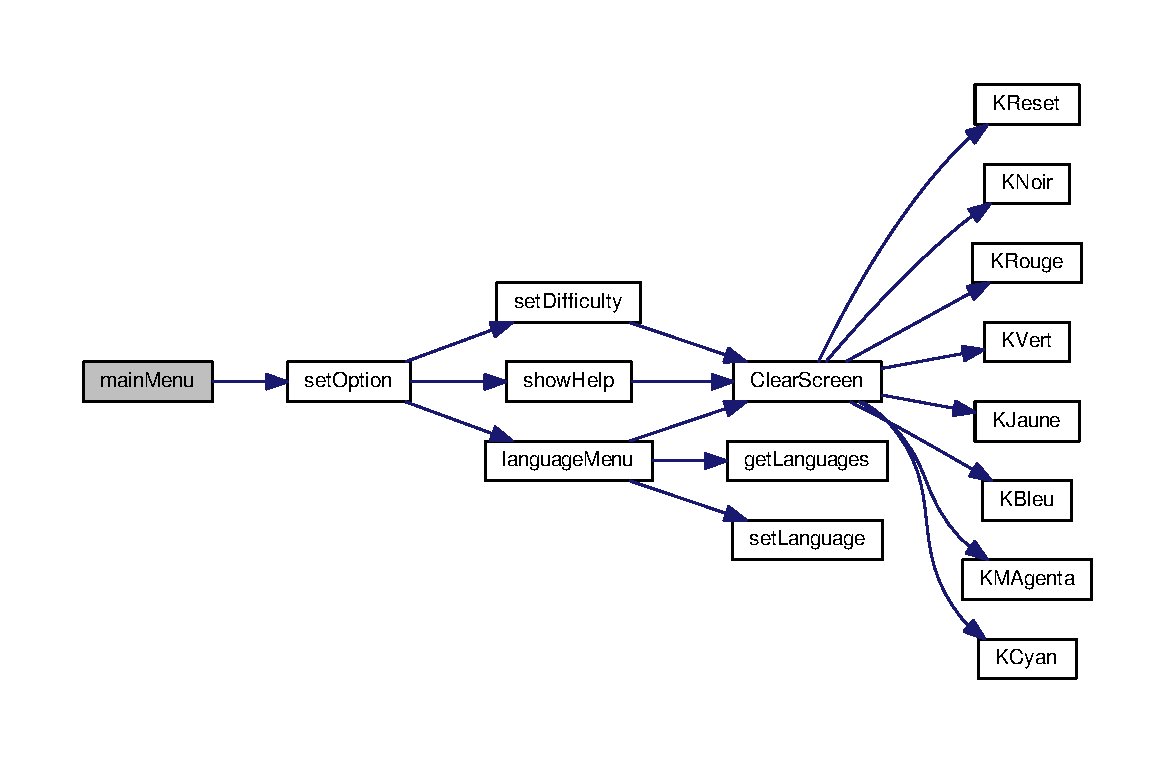
\includegraphics[width=350pt]{main_8cpp_aaed5cc5349863a6b8a7a86c74f28263a_cgraph}
\end{center}
\end{figure}




Here is the caller graph for this function\+:\nopagebreak
\begin{figure}[H]
\begin{center}
\leavevmode
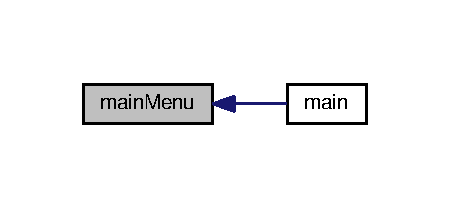
\includegraphics[width=216pt]{main_8cpp_aaed5cc5349863a6b8a7a86c74f28263a_icgraph}
\end{center}
\end{figure}


\index{main.\+cpp@{main.\+cpp}!Move\+Token@{Move\+Token}}
\index{Move\+Token@{Move\+Token}!main.\+cpp@{main.\+cpp}}
\subsubsection[{\texorpdfstring{Move\+Token(\+C\+Matrix \&\+Mat, char Move, C\+Position \&\+Pos)}{MoveToken(CMatrix &Mat, char Move, CPosition &Pos)}}]{\setlength{\rightskip}{0pt plus 5cm}void Move\+Token (
\begin{DoxyParamCaption}
\item[{{\bf C\+Matrix} \&}]{Mat, }
\item[{char}]{Move, }
\item[{{\bf C\+Position} \&}]{Pos}
\end{DoxyParamCaption}
)}\hypertarget{main_8cpp_adb6ae9f5ad188e663124a9afa23467bf}{}\label{main_8cpp_adb6ae9f5ad188e663124a9afa23467bf}


Deplace un joueur. 


\begin{DoxyParams}{Parameters}
{\em Grille} & du jeu \\
\hline
{\em Caractere} & saisi au clavier \\
\hline
{\em Position} & du joueur \\
\hline
\end{DoxyParams}


Here is the call graph for this function\+:
\nopagebreak
\begin{figure}[H]
\begin{center}
\leavevmode
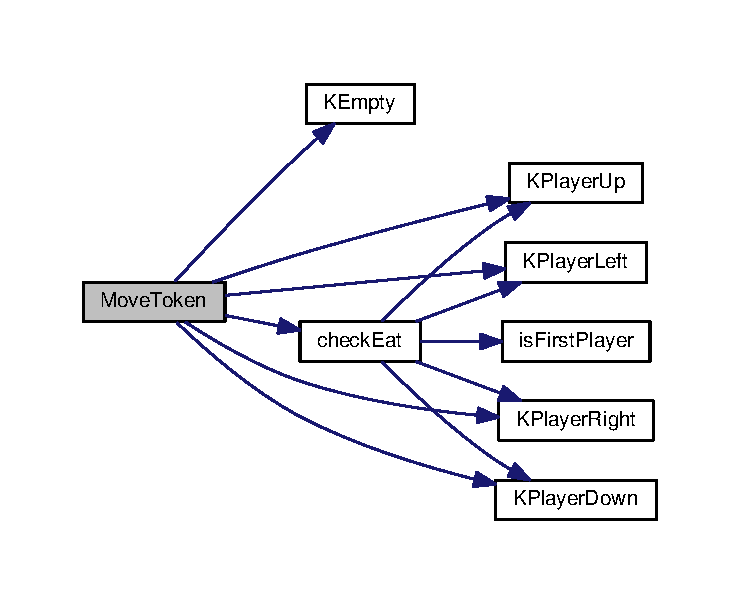
\includegraphics[width=350pt]{main_8cpp_adb6ae9f5ad188e663124a9afa23467bf_cgraph}
\end{center}
\end{figure}




Here is the caller graph for this function\+:\nopagebreak
\begin{figure}[H]
\begin{center}
\leavevmode
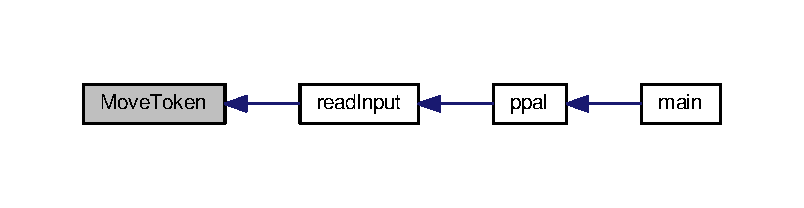
\includegraphics[width=350pt]{main_8cpp_adb6ae9f5ad188e663124a9afa23467bf_icgraph}
\end{center}
\end{figure}


\index{main.\+cpp@{main.\+cpp}!play\+Music@{play\+Music}}
\index{play\+Music@{play\+Music}!main.\+cpp@{main.\+cpp}}
\subsubsection[{\texorpdfstring{play\+Music()}{playMusic()}}]{\setlength{\rightskip}{0pt plus 5cm}void play\+Music (
\begin{DoxyParamCaption}
{}
\end{DoxyParamCaption}
)}\hypertarget{main_8cpp_a5950f90fdf5f67fab5bae67d2b350de9}{}\label{main_8cpp_a5950f90fdf5f67fab5bae67d2b350de9}


Fonction pour jouer la musique. 



Here is the caller graph for this function\+:\nopagebreak
\begin{figure}[H]
\begin{center}
\leavevmode
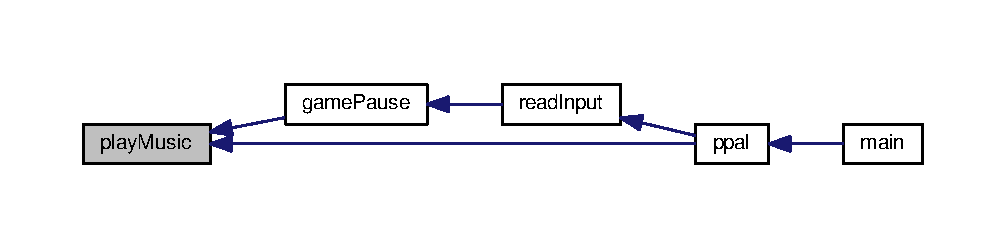
\includegraphics[width=350pt]{main_8cpp_a5950f90fdf5f67fab5bae67d2b350de9_icgraph}
\end{center}
\end{figure}


\index{main.\+cpp@{main.\+cpp}!pop\+Food@{pop\+Food}}
\index{pop\+Food@{pop\+Food}!main.\+cpp@{main.\+cpp}}
\subsubsection[{\texorpdfstring{pop\+Food(\+C\+Matrix \&\+Mat)}{popFood(CMatrix &Mat)}}]{\setlength{\rightskip}{0pt plus 5cm}void pop\+Food (
\begin{DoxyParamCaption}
\item[{{\bf C\+Matrix} \&}]{Mat}
\end{DoxyParamCaption}
)}\hypertarget{main_8cpp_a3d6a81a68086b8f60d124449ebca3ba1}{}\label{main_8cpp_a3d6a81a68086b8f60d124449ebca3ba1}


Fait apparaitre un tresor dans la grille si les conditions sont remplies. 


\begin{DoxyParams}{Parameters}
{\em La} & grille du jeu \\
\hline
\end{DoxyParams}


Here is the caller graph for this function\+:\nopagebreak
\begin{figure}[H]
\begin{center}
\leavevmode
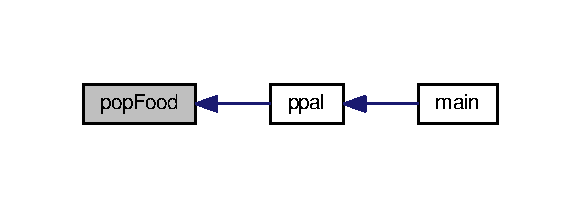
\includegraphics[width=279pt]{main_8cpp_a3d6a81a68086b8f60d124449ebca3ba1_icgraph}
\end{center}
\end{figure}


\index{main.\+cpp@{main.\+cpp}!ppal@{ppal}}
\index{ppal@{ppal}!main.\+cpp@{main.\+cpp}}
\subsubsection[{\texorpdfstring{ppal()}{ppal()}}]{\setlength{\rightskip}{0pt plus 5cm}bool ppal (
\begin{DoxyParamCaption}
{}
\end{DoxyParamCaption}
)}\hypertarget{main_8cpp_af5049d09a64bd19378a243787b57d027}{}\label{main_8cpp_af5049d09a64bd19378a243787b57d027}


Fonction principale, contient la boucle de jeu. 

\begin{DoxyReturn}{Returns}
Si le joueur veut continuer ou non 
\end{DoxyReturn}


Here is the call graph for this function\+:
\nopagebreak
\begin{figure}[H]
\begin{center}
\leavevmode
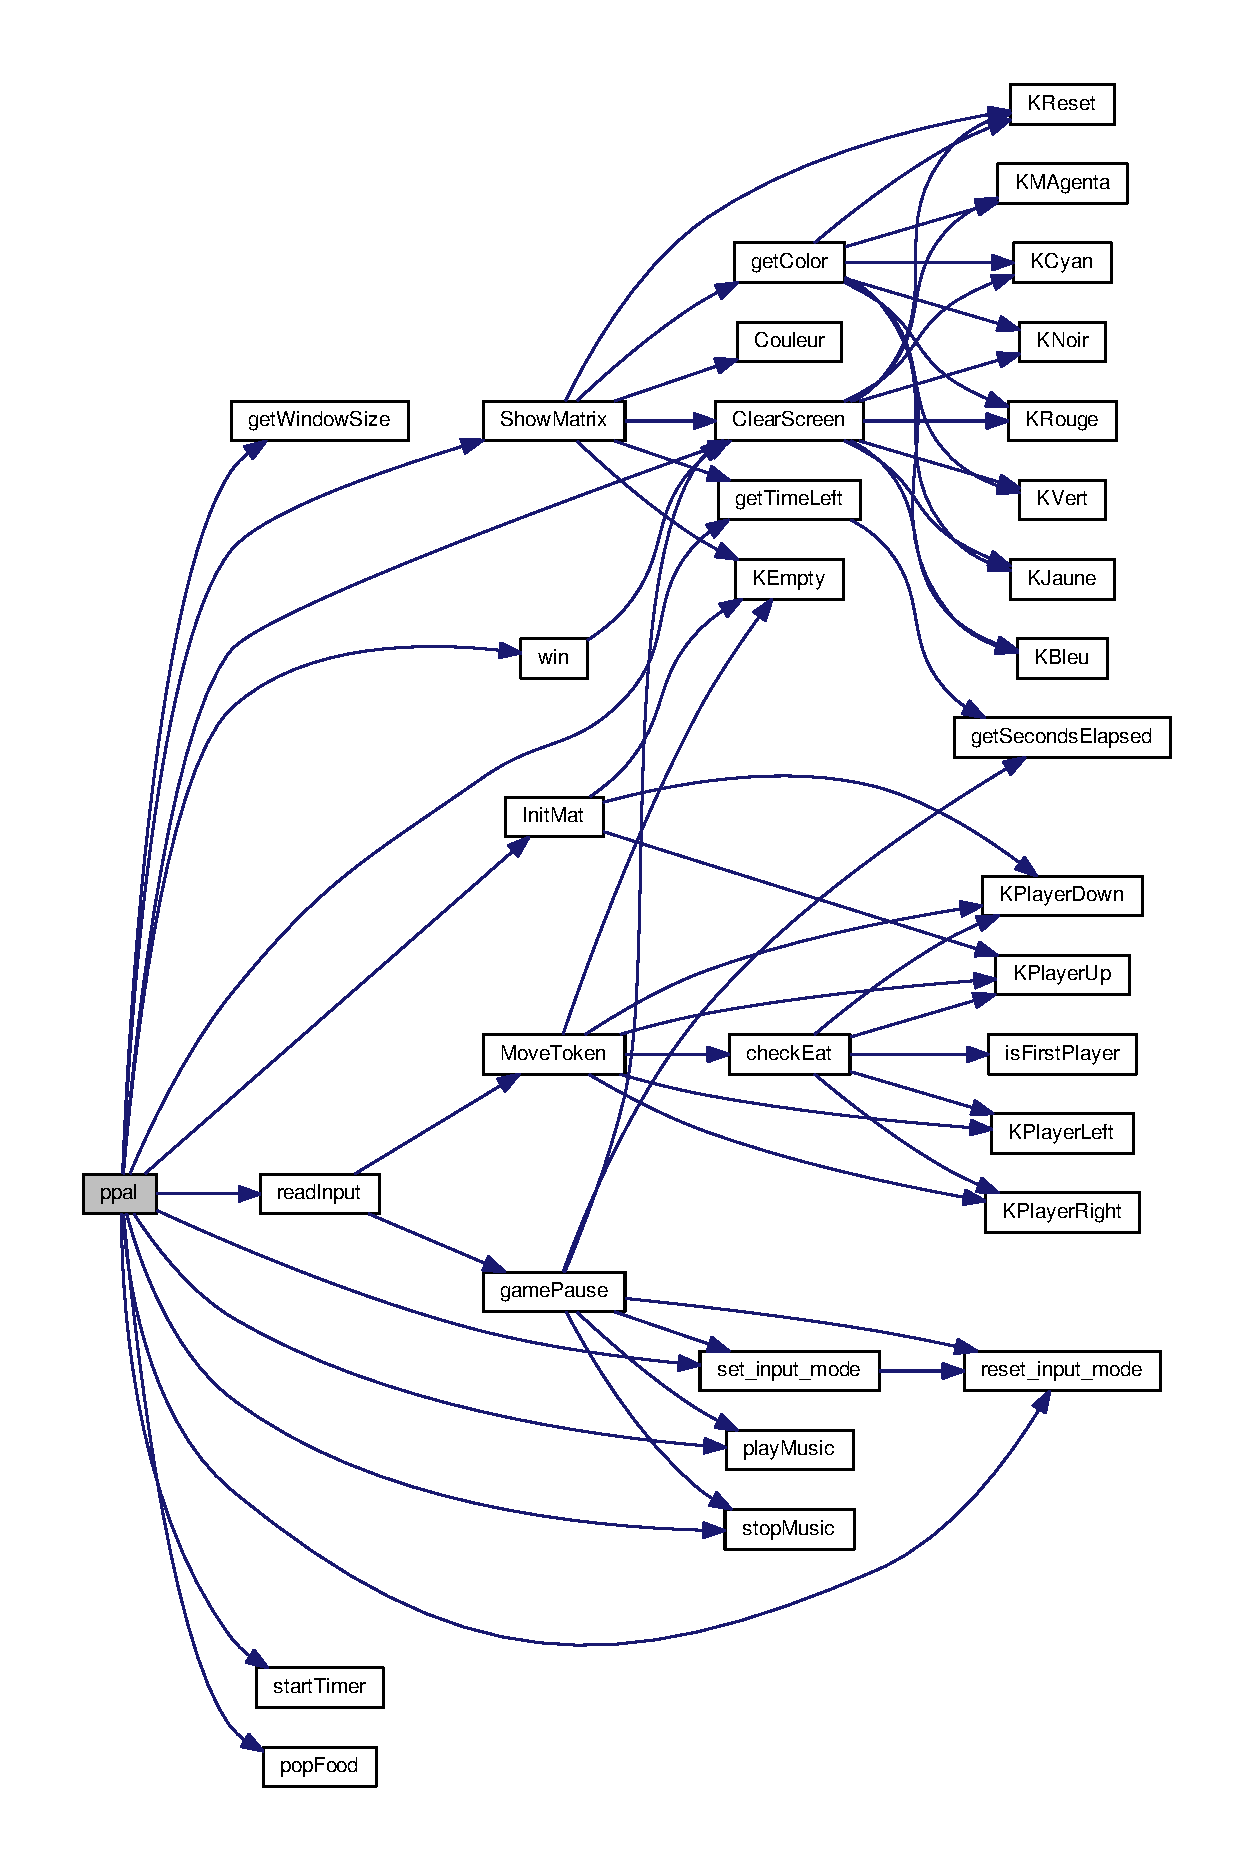
\includegraphics[width=350pt]{main_8cpp_af5049d09a64bd19378a243787b57d027_cgraph}
\end{center}
\end{figure}




Here is the caller graph for this function\+:\nopagebreak
\begin{figure}[H]
\begin{center}
\leavevmode
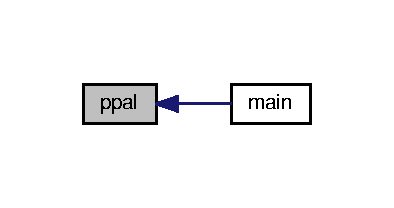
\includegraphics[width=189pt]{main_8cpp_af5049d09a64bd19378a243787b57d027_icgraph}
\end{center}
\end{figure}


\index{main.\+cpp@{main.\+cpp}!read\+Input@{read\+Input}}
\index{read\+Input@{read\+Input}!main.\+cpp@{main.\+cpp}}
\subsubsection[{\texorpdfstring{read\+Input(char \&\+Input)}{readInput(char &Input)}}]{\setlength{\rightskip}{0pt plus 5cm}void read\+Input (
\begin{DoxyParamCaption}
\item[{char \&}]{Input}
\end{DoxyParamCaption}
)}\hypertarget{main_8cpp_a6df6aa26bcfa8c1d0fcda8b8b8075abc}{}\label{main_8cpp_a6df6aa26bcfa8c1d0fcda8b8b8075abc}


Lis la saisie clavier. 


\begin{DoxyParams}{Parameters}
{\em Saisie} & du clavier \\
\hline
\end{DoxyParams}


Here is the call graph for this function\+:
\nopagebreak
\begin{figure}[H]
\begin{center}
\leavevmode
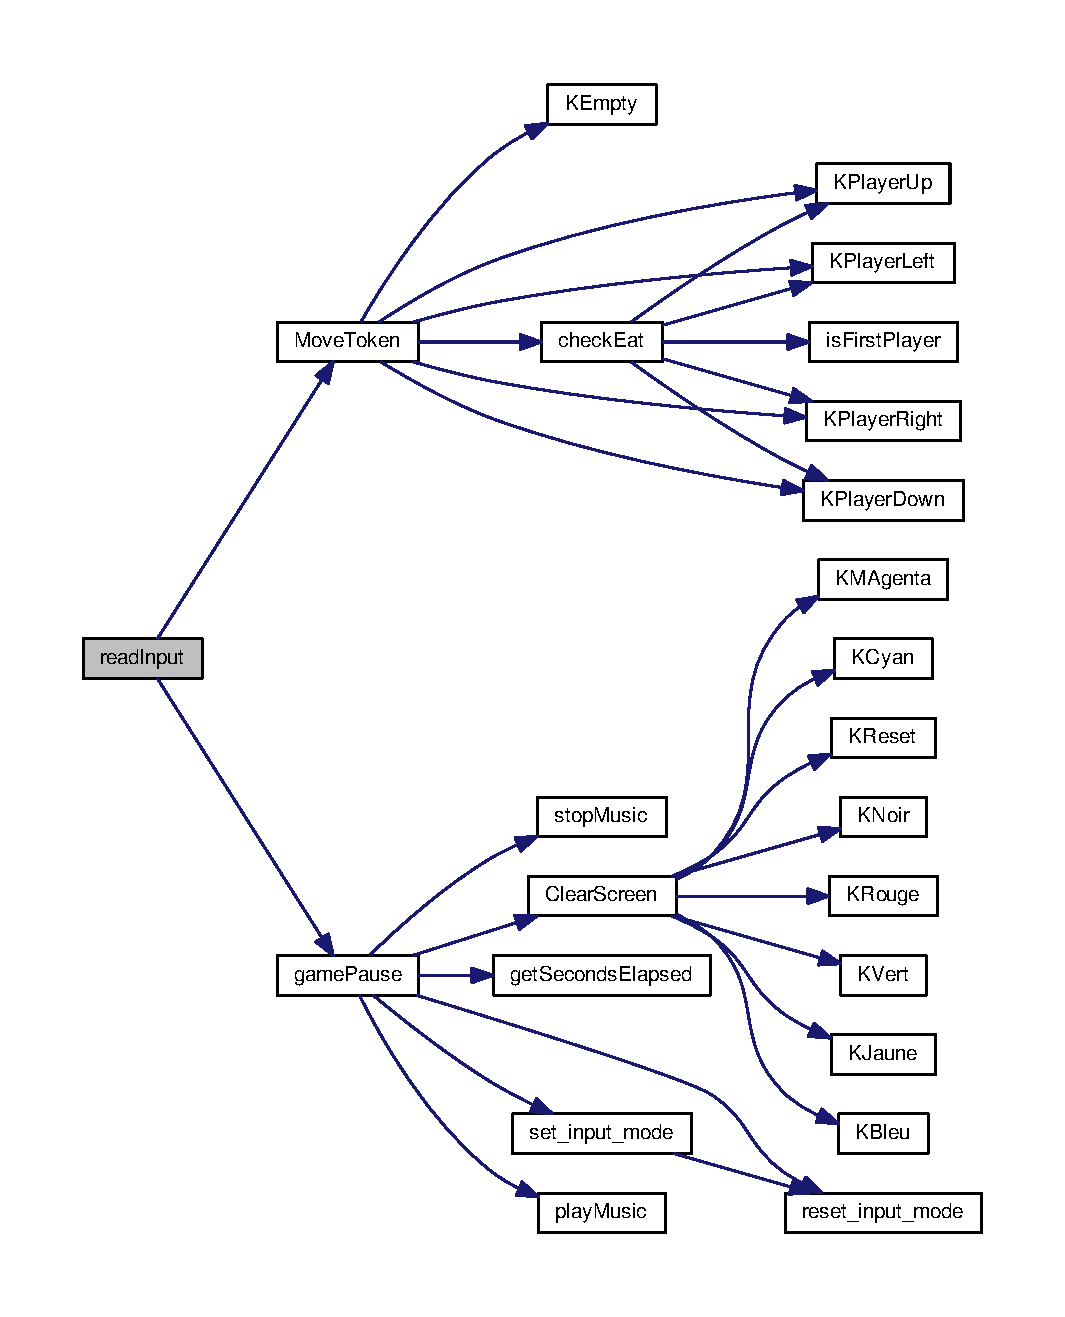
\includegraphics[width=350pt]{main_8cpp_a6df6aa26bcfa8c1d0fcda8b8b8075abc_cgraph}
\end{center}
\end{figure}




Here is the caller graph for this function\+:\nopagebreak
\begin{figure}[H]
\begin{center}
\leavevmode
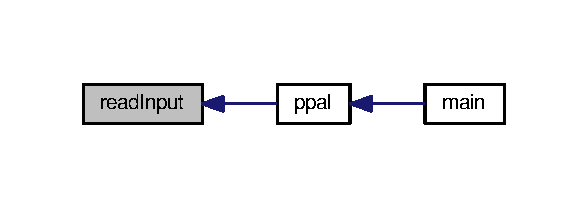
\includegraphics[width=282pt]{main_8cpp_a6df6aa26bcfa8c1d0fcda8b8b8075abc_icgraph}
\end{center}
\end{figure}


\index{main.\+cpp@{main.\+cpp}!reset\+\_\+input\+\_\+mode@{reset\+\_\+input\+\_\+mode}}
\index{reset\+\_\+input\+\_\+mode@{reset\+\_\+input\+\_\+mode}!main.\+cpp@{main.\+cpp}}
\subsubsection[{\texorpdfstring{reset\+\_\+input\+\_\+mode(void)}{reset_input_mode(void)}}]{\setlength{\rightskip}{0pt plus 5cm}void reset\+\_\+input\+\_\+mode (
\begin{DoxyParamCaption}
\item[{void}]{}
\end{DoxyParamCaption}
)}\hypertarget{main_8cpp_af99d8c0775d8c342a142e2be8c2ea592}{}\label{main_8cpp_af99d8c0775d8c342a142e2be8c2ea592}


Remet le mode d\textquotesingle{}entree par defaut du programme. 



Here is the caller graph for this function\+:\nopagebreak
\begin{figure}[H]
\begin{center}
\leavevmode
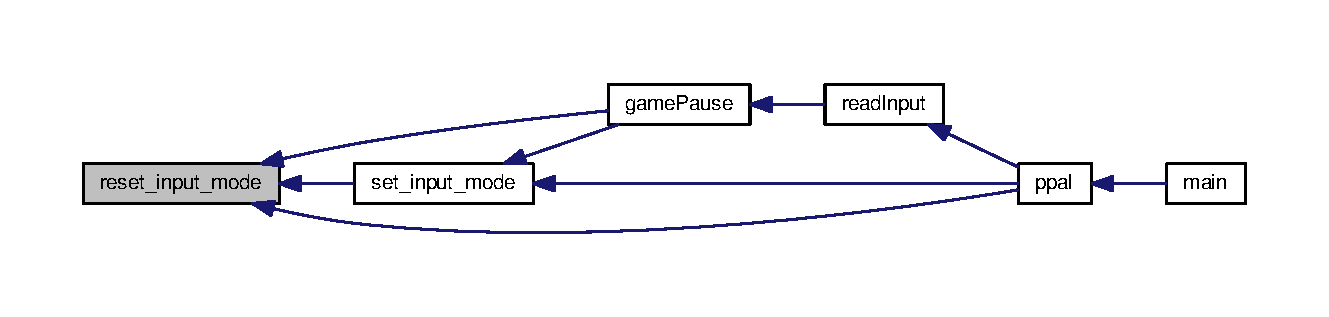
\includegraphics[width=350pt]{main_8cpp_af99d8c0775d8c342a142e2be8c2ea592_icgraph}
\end{center}
\end{figure}


\index{main.\+cpp@{main.\+cpp}!set\+\_\+input\+\_\+mode@{set\+\_\+input\+\_\+mode}}
\index{set\+\_\+input\+\_\+mode@{set\+\_\+input\+\_\+mode}!main.\+cpp@{main.\+cpp}}
\subsubsection[{\texorpdfstring{set\+\_\+input\+\_\+mode(void)}{set_input_mode(void)}}]{\setlength{\rightskip}{0pt plus 5cm}void set\+\_\+input\+\_\+mode (
\begin{DoxyParamCaption}
\item[{void}]{}
\end{DoxyParamCaption}
)}\hypertarget{main_8cpp_a224cd3d46cfe5381606415ce3585b91f}{}\label{main_8cpp_a224cd3d46cfe5381606415ce3585b91f}


Change le mode d\textquotesingle{}entree en mode non canonique. 



Here is the call graph for this function\+:\nopagebreak
\begin{figure}[H]
\begin{center}
\leavevmode
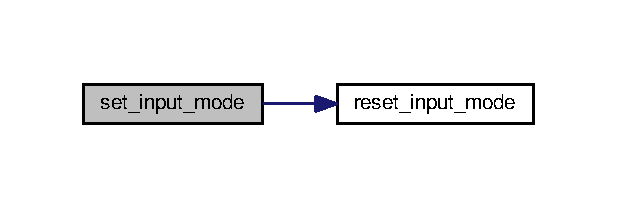
\includegraphics[width=296pt]{main_8cpp_a224cd3d46cfe5381606415ce3585b91f_cgraph}
\end{center}
\end{figure}




Here is the caller graph for this function\+:\nopagebreak
\begin{figure}[H]
\begin{center}
\leavevmode
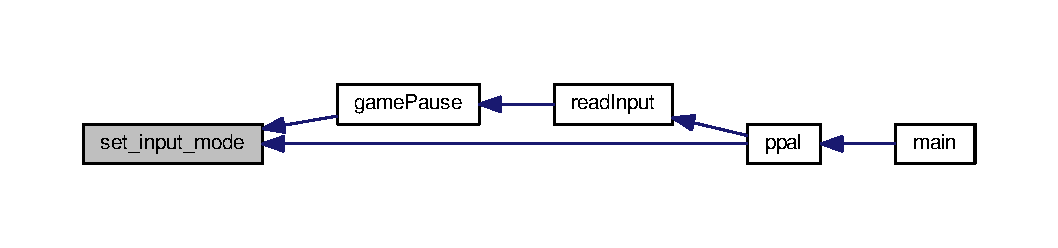
\includegraphics[width=350pt]{main_8cpp_a224cd3d46cfe5381606415ce3585b91f_icgraph}
\end{center}
\end{figure}


\index{main.\+cpp@{main.\+cpp}!set\+Defaults@{set\+Defaults}}
\index{set\+Defaults@{set\+Defaults}!main.\+cpp@{main.\+cpp}}
\subsubsection[{\texorpdfstring{set\+Defaults(\+C\+My\+Param \&\+My\+Params)}{setDefaults(CMyParam &MyParams)}}]{\setlength{\rightskip}{0pt plus 5cm}void set\+Defaults (
\begin{DoxyParamCaption}
\item[{{\bf C\+My\+Param} \&}]{My\+Params}
\end{DoxyParamCaption}
)}\hypertarget{main_8cpp_a0f82957da2c48a8760217ffec9b8fb3e}{}\label{main_8cpp_a0f82957da2c48a8760217ffec9b8fb3e}


Definit quelques parametres par defaut. 


\begin{DoxyParams}{Parameters}
{\em Parametres} & du jeu \\
\hline
\end{DoxyParams}


Here is the caller graph for this function\+:\nopagebreak
\begin{figure}[H]
\begin{center}
\leavevmode
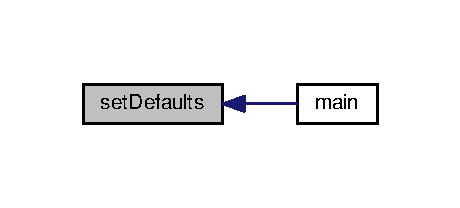
\includegraphics[width=221pt]{main_8cpp_a0f82957da2c48a8760217ffec9b8fb3e_icgraph}
\end{center}
\end{figure}


\index{main.\+cpp@{main.\+cpp}!set\+Difficulty@{set\+Difficulty}}
\index{set\+Difficulty@{set\+Difficulty}!main.\+cpp@{main.\+cpp}}
\subsubsection[{\texorpdfstring{set\+Difficulty()}{setDifficulty()}}]{\setlength{\rightskip}{0pt plus 5cm}void set\+Difficulty (
\begin{DoxyParamCaption}
{}
\end{DoxyParamCaption}
)}\hypertarget{main_8cpp_a28af16941c845fe85c0ad486f67928c1}{}\label{main_8cpp_a28af16941c845fe85c0ad486f67928c1}


Affiche le menu de selection de la difficulte. 



Here is the call graph for this function\+:\nopagebreak
\begin{figure}[H]
\begin{center}
\leavevmode
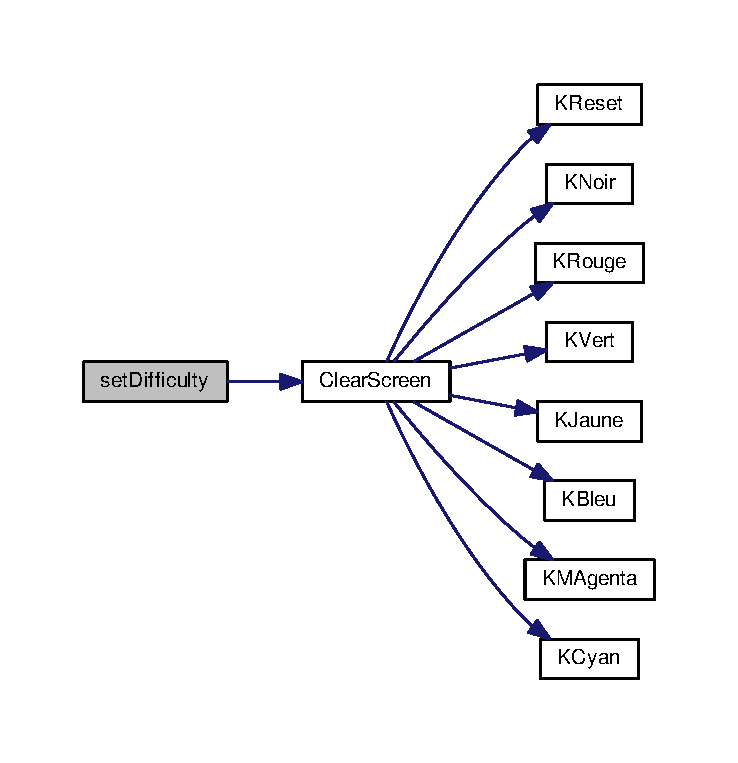
\includegraphics[width=350pt]{main_8cpp_a28af16941c845fe85c0ad486f67928c1_cgraph}
\end{center}
\end{figure}




Here is the caller graph for this function\+:\nopagebreak
\begin{figure}[H]
\begin{center}
\leavevmode
\includegraphics[width=350pt]{main_8cpp_a28af16941c845fe85c0ad486f67928c1_icgraph}
\end{center}
\end{figure}


\index{main.\+cpp@{main.\+cpp}!set\+Language@{set\+Language}}
\index{set\+Language@{set\+Language}!main.\+cpp@{main.\+cpp}}
\subsubsection[{\texorpdfstring{set\+Language(string \&\+Language\+File)}{setLanguage(string &LanguageFile)}}]{\setlength{\rightskip}{0pt plus 5cm}void set\+Language (
\begin{DoxyParamCaption}
\item[{string \&}]{Language\+File}
\end{DoxyParamCaption}
)}\hypertarget{main_8cpp_a6a5bd3703942c1006576ceb0ef614a91}{}\label{main_8cpp_a6a5bd3703942c1006576ceb0ef614a91}


Definit la langue du jeu. 


\begin{DoxyParams}{Parameters}
{\em Le} & nom du fichier qui contient les parametres de langue \\
\hline
\end{DoxyParams}


Here is the caller graph for this function\+:\nopagebreak
\begin{figure}[H]
\begin{center}
\leavevmode
\includegraphics[width=350pt]{main_8cpp_a6a5bd3703942c1006576ceb0ef614a91_icgraph}
\end{center}
\end{figure}


\index{main.\+cpp@{main.\+cpp}!set\+Language\+From\+Locale@{set\+Language\+From\+Locale}}
\index{set\+Language\+From\+Locale@{set\+Language\+From\+Locale}!main.\+cpp@{main.\+cpp}}
\subsubsection[{\texorpdfstring{set\+Language\+From\+Locale(string \&\+Locale)}{setLanguageFromLocale(string &Locale)}}]{\setlength{\rightskip}{0pt plus 5cm}void set\+Language\+From\+Locale (
\begin{DoxyParamCaption}
\item[{string \&}]{Locale}
\end{DoxyParamCaption}
)}\hypertarget{main_8cpp_a8738b59733022baef4ff40e331c09554}{}\label{main_8cpp_a8738b59733022baef4ff40e331c09554}


Definit la langue du jeu a partir d\textquotesingle{}une locale. 


\begin{DoxyParams}{Parameters}
{\em La} & locale de la langue a changer \\
\hline
\end{DoxyParams}


Here is the call graph for this function\+:\nopagebreak
\begin{figure}[H]
\begin{center}
\leavevmode
\includegraphics[width=316pt]{main_8cpp_a8738b59733022baef4ff40e331c09554_cgraph}
\end{center}
\end{figure}




Here is the caller graph for this function\+:\nopagebreak
\begin{figure}[H]
\begin{center}
\leavevmode
\includegraphics[width=350pt]{main_8cpp_a8738b59733022baef4ff40e331c09554_icgraph}
\end{center}
\end{figure}


\index{main.\+cpp@{main.\+cpp}!set\+Option@{set\+Option}}
\index{set\+Option@{set\+Option}!main.\+cpp@{main.\+cpp}}
\subsubsection[{\texorpdfstring{set\+Option(int \&\+Choix)}{setOption(int &Choix)}}]{\setlength{\rightskip}{0pt plus 5cm}bool set\+Option (
\begin{DoxyParamCaption}
\item[{int \&}]{Choix}
\end{DoxyParamCaption}
)}\hypertarget{main_8cpp_ad8588f4f4d24ec38f448e679a68cd62f}{}\label{main_8cpp_ad8588f4f4d24ec38f448e679a68cd62f}


Regle l\textquotesingle{}option selectionnee. 


\begin{DoxyParams}{Parameters}
{\em Option} & a regler \\
\hline
\end{DoxyParams}
\begin{DoxyReturn}{Returns}
Si le joueur est pret a jouer ou non 
\end{DoxyReturn}


Here is the call graph for this function\+:\nopagebreak
\begin{figure}[H]
\begin{center}
\leavevmode
\includegraphics[width=350pt]{main_8cpp_ad8588f4f4d24ec38f448e679a68cd62f_cgraph}
\end{center}
\end{figure}




Here is the caller graph for this function\+:\nopagebreak
\begin{figure}[H]
\begin{center}
\leavevmode
\includegraphics[width=311pt]{main_8cpp_ad8588f4f4d24ec38f448e679a68cd62f_icgraph}
\end{center}
\end{figure}


\index{main.\+cpp@{main.\+cpp}!show\+Help@{show\+Help}}
\index{show\+Help@{show\+Help}!main.\+cpp@{main.\+cpp}}
\subsubsection[{\texorpdfstring{show\+Help()}{showHelp()}}]{\setlength{\rightskip}{0pt plus 5cm}void show\+Help (
\begin{DoxyParamCaption}
{}
\end{DoxyParamCaption}
)}\hypertarget{main_8cpp_aec315d77f5c38417289a0e311d2a9d31}{}\label{main_8cpp_aec315d77f5c38417289a0e311d2a9d31}


Affiche le fichier d\textquotesingle{}aide. 



Here is the call graph for this function\+:\nopagebreak
\begin{figure}[H]
\begin{center}
\leavevmode
\includegraphics[width=345pt]{main_8cpp_aec315d77f5c38417289a0e311d2a9d31_cgraph}
\end{center}
\end{figure}




Here is the caller graph for this function\+:\nopagebreak
\begin{figure}[H]
\begin{center}
\leavevmode
\includegraphics[width=350pt]{main_8cpp_aec315d77f5c38417289a0e311d2a9d31_icgraph}
\end{center}
\end{figure}


\index{main.\+cpp@{main.\+cpp}!Show\+Matrix@{Show\+Matrix}}
\index{Show\+Matrix@{Show\+Matrix}!main.\+cpp@{main.\+cpp}}
\subsubsection[{\texorpdfstring{Show\+Matrix(const C\+Matrix \&\+Mat)}{ShowMatrix(const CMatrix &Mat)}}]{\setlength{\rightskip}{0pt plus 5cm}void Show\+Matrix (
\begin{DoxyParamCaption}
\item[{const {\bf C\+Matrix} \&}]{Mat}
\end{DoxyParamCaption}
)}\hypertarget{main_8cpp_aa1e1ee1a111de597ed2250892119fad2}{}\label{main_8cpp_aa1e1ee1a111de597ed2250892119fad2}


Affiche l\textquotesingle{}interface principale du jeu. 


\begin{DoxyParams}{Parameters}
{\em La} & grille a afficher \\
\hline
\end{DoxyParams}


Here is the call graph for this function\+:\nopagebreak
\begin{figure}[H]
\begin{center}
\leavevmode
\includegraphics[width=350pt]{main_8cpp_aa1e1ee1a111de597ed2250892119fad2_cgraph}
\end{center}
\end{figure}




Here is the caller graph for this function\+:\nopagebreak
\begin{figure}[H]
\begin{center}
\leavevmode
\includegraphics[width=293pt]{main_8cpp_aa1e1ee1a111de597ed2250892119fad2_icgraph}
\end{center}
\end{figure}


\index{main.\+cpp@{main.\+cpp}!start\+Timer@{start\+Timer}}
\index{start\+Timer@{start\+Timer}!main.\+cpp@{main.\+cpp}}
\subsubsection[{\texorpdfstring{start\+Timer()}{startTimer()}}]{\setlength{\rightskip}{0pt plus 5cm}void start\+Timer (
\begin{DoxyParamCaption}
{}
\end{DoxyParamCaption}
)}\hypertarget{main_8cpp_aec53975ffc59ffaf3080db21af0d2f6e}{}\label{main_8cpp_aec53975ffc59ffaf3080db21af0d2f6e}


Démarre le chronomètre. 



Here is the caller graph for this function\+:\nopagebreak
\begin{figure}[H]
\begin{center}
\leavevmode
\includegraphics[width=286pt]{main_8cpp_aec53975ffc59ffaf3080db21af0d2f6e_icgraph}
\end{center}
\end{figure}


\index{main.\+cpp@{main.\+cpp}!stop\+Music@{stop\+Music}}
\index{stop\+Music@{stop\+Music}!main.\+cpp@{main.\+cpp}}
\subsubsection[{\texorpdfstring{stop\+Music()}{stopMusic()}}]{\setlength{\rightskip}{0pt plus 5cm}void stop\+Music (
\begin{DoxyParamCaption}
{}
\end{DoxyParamCaption}
)}\hypertarget{main_8cpp_a7473e9a04dc2e8f05241857d86586194}{}\label{main_8cpp_a7473e9a04dc2e8f05241857d86586194}


Fonction pour arreter la musique. 



Here is the caller graph for this function\+:\nopagebreak
\begin{figure}[H]
\begin{center}
\leavevmode
\includegraphics[width=350pt]{main_8cpp_a7473e9a04dc2e8f05241857d86586194_icgraph}
\end{center}
\end{figure}


\index{main.\+cpp@{main.\+cpp}!win@{win}}
\index{win@{win}!main.\+cpp@{main.\+cpp}}
\subsubsection[{\texorpdfstring{win(unsigned Player, unsigned \&\+Score1, unsigned \&\+Score2)}{win(unsigned Player, unsigned &Score1, unsigned &Score2)}}]{\setlength{\rightskip}{0pt plus 5cm}bool win (
\begin{DoxyParamCaption}
\item[{unsigned}]{Player, }
\item[{unsigned \&}]{Score1, }
\item[{unsigned \&}]{Score2}
\end{DoxyParamCaption}
)}\hypertarget{main_8cpp_a1ad2098fbb826463ee14c62abf400789}{}\label{main_8cpp_a1ad2098fbb826463ee14c62abf400789}


Fonction appelee a la fin du jeu, pour afficher le gagnant. 


\begin{DoxyParams}{Parameters}
{\em Le} & joueur gagnant \\
\hline
{\em Le} & score du gagnant \\
\hline
{\em Le} & score du perdant \\
\hline
\end{DoxyParams}
\begin{DoxyReturn}{Returns}
Si le joueur veut rejouer ou non 
\end{DoxyReturn}


Here is the call graph for this function\+:\nopagebreak
\begin{figure}[H]
\begin{center}
\leavevmode
\includegraphics[width=317pt]{main_8cpp_a1ad2098fbb826463ee14c62abf400789_cgraph}
\end{center}
\end{figure}




Here is the caller graph for this function\+:\nopagebreak
\begin{figure}[H]
\begin{center}
\leavevmode
\includegraphics[width=257pt]{main_8cpp_a1ad2098fbb826463ee14c62abf400789_icgraph}
\end{center}
\end{figure}




\subsection{Variable Documentation}
\index{main.\+cpp@{main.\+cpp}!food\+Setting@{food\+Setting}}
\index{food\+Setting@{food\+Setting}!main.\+cpp@{main.\+cpp}}
\subsubsection[{\texorpdfstring{food\+Setting}{foodSetting}}]{\setlength{\rightskip}{0pt plus 5cm}const string food\+Setting = \char`\"{}food\char`\"{}}\hypertarget{main_8cpp_aa438f6e616364aa2fd7eae4b2d2679aa}{}\label{main_8cpp_aa438f6e616364aa2fd7eae4b2d2679aa}


Option du trésor a \char`\"{}manger\char`\"{}. 

\index{main.\+cpp@{main.\+cpp}!language\+Setting@{language\+Setting}}
\index{language\+Setting@{language\+Setting}!main.\+cpp@{main.\+cpp}}
\subsubsection[{\texorpdfstring{language\+Setting}{languageSetting}}]{\setlength{\rightskip}{0pt plus 5cm}const string language\+Setting = \char`\"{}langue\char`\"{}}\hypertarget{main_8cpp_a2051b3676c604790f8de1af336cf03ff}{}\label{main_8cpp_a2051b3676c604790f8de1af336cf03ff}


Option de langue. 

\index{main.\+cpp@{main.\+cpp}!Mat@{Mat}}
\index{Mat@{Mat}!main.\+cpp@{main.\+cpp}}
\subsubsection[{\texorpdfstring{Mat}{Mat}}]{\setlength{\rightskip}{0pt plus 5cm}{\bf C\+Matrix} Mat}\hypertarget{main_8cpp_a9a550e23325a7e17e559150dce3994c9}{}\label{main_8cpp_a9a550e23325a7e17e559150dce3994c9}


Grille de jeu. 

\index{main.\+cpp@{main.\+cpp}!Player1@{Player1}}
\index{Player1@{Player1}!main.\+cpp@{main.\+cpp}}
\subsubsection[{\texorpdfstring{Player1}{Player1}}]{\setlength{\rightskip}{0pt plus 5cm}{\bf C\+Position} Player1}\hypertarget{main_8cpp_ae60f372c980f382cde2766b604e02bad}{}\label{main_8cpp_ae60f372c980f382cde2766b604e02bad}


Position du joueur 1. 

\index{main.\+cpp@{main.\+cpp}!Player2@{Player2}}
\index{Player2@{Player2}!main.\+cpp@{main.\+cpp}}
\subsubsection[{\texorpdfstring{Player2}{Player2}}]{\setlength{\rightskip}{0pt plus 5cm}{\bf C\+Position} Player2}\hypertarget{main_8cpp_aec8bb76921a4ecfabdfe38d63f1ba46e}{}\label{main_8cpp_aec8bb76921a4ecfabdfe38d63f1ba46e}


Position du joueur 2. 

\index{main.\+cpp@{main.\+cpp}!random\+Counter@{random\+Counter}}
\index{random\+Counter@{random\+Counter}!main.\+cpp@{main.\+cpp}}
\subsubsection[{\texorpdfstring{random\+Counter}{randomCounter}}]{\setlength{\rightskip}{0pt plus 5cm}unsigned random\+Counter = 0}\hypertarget{main_8cpp_af22e57743571134d7814f755c757f01f}{}\label{main_8cpp_af22e57743571134d7814f755c757f01f}


Compteur du generateur aleatoire. 

\index{main.\+cpp@{main.\+cpp}!saved\+\_\+attributes@{saved\+\_\+attributes}}
\index{saved\+\_\+attributes@{saved\+\_\+attributes}!main.\+cpp@{main.\+cpp}}
\subsubsection[{\texorpdfstring{saved\+\_\+attributes}{saved_attributes}}]{\setlength{\rightskip}{0pt plus 5cm}struct termios saved\+\_\+attributes}\hypertarget{main_8cpp_a23564a19f1e34105cc4892cab4108bf4}{}\label{main_8cpp_a23564a19f1e34105cc4892cab4108bf4}


Configuration du terminal, notemment le mode d\textquotesingle{}entrée. 

\index{main.\+cpp@{main.\+cpp}!Score\+J1@{Score\+J1}}
\index{Score\+J1@{Score\+J1}!main.\+cpp@{main.\+cpp}}
\subsubsection[{\texorpdfstring{Score\+J1}{ScoreJ1}}]{\setlength{\rightskip}{0pt plus 5cm}unsigned Score\+J1}\hypertarget{main_8cpp_a5c818c44818d411efb8d4959642de080}{}\label{main_8cpp_a5c818c44818d411efb8d4959642de080}


Score du joueur 1. 

\index{main.\+cpp@{main.\+cpp}!Score\+J2@{Score\+J2}}
\index{Score\+J2@{Score\+J2}!main.\+cpp@{main.\+cpp}}
\subsubsection[{\texorpdfstring{Score\+J2}{ScoreJ2}}]{\setlength{\rightskip}{0pt plus 5cm}unsigned Score\+J2}\hypertarget{main_8cpp_a4275f4e3e4da025275d2b467e56e569c}{}\label{main_8cpp_a4275f4e3e4da025275d2b467e56e569c}


Score du joueur 2. 

\index{main.\+cpp@{main.\+cpp}!Settings@{Settings}}
\index{Settings@{Settings}!main.\+cpp@{main.\+cpp}}
\subsubsection[{\texorpdfstring{Settings}{Settings}}]{\setlength{\rightskip}{0pt plus 5cm}{\bf C\+My\+Param} Settings}\hypertarget{main_8cpp_a59504f224e8084089ed8eeab31e9afe3}{}\label{main_8cpp_a59504f224e8084089ed8eeab31e9afe3}


Réglages du jeu. 

\index{main.\+cpp@{main.\+cpp}!Time@{Time}}
\index{Time@{Time}!main.\+cpp@{main.\+cpp}}
\subsubsection[{\texorpdfstring{Time}{Time}}]{\setlength{\rightskip}{0pt plus 5cm}unsigned long Time}\hypertarget{main_8cpp_a08a45f88d378775661ab944edf9fded5}{}\label{main_8cpp_a08a45f88d378775661ab944edf9fded5}


Temps au debut du chronometre. 

\index{main.\+cpp@{main.\+cpp}!V\+Colors@{V\+Colors}}
\index{V\+Colors@{V\+Colors}!main.\+cpp@{main.\+cpp}}
\subsubsection[{\texorpdfstring{V\+Colors}{VColors}}]{\setlength{\rightskip}{0pt plus 5cm}const vector$<$string$>$ V\+Colors \{\char`\"{}Color\+Player1\char`\"{}, \char`\"{}Color\+Player2\char`\"{},\char`\"{}Color\+Food\char`\"{}\}}\hypertarget{main_8cpp_a95c4ac81b0b4391b2e9761ab491edd15}{}\label{main_8cpp_a95c4ac81b0b4391b2e9761ab491edd15}


Liste des options de couleur. 

\index{main.\+cpp@{main.\+cpp}!V\+Controls@{V\+Controls}}
\index{V\+Controls@{V\+Controls}!main.\+cpp@{main.\+cpp}}
\subsubsection[{\texorpdfstring{V\+Controls}{VControls}}]{\setlength{\rightskip}{0pt plus 5cm}const vector$<$string$>$ V\+Controls \{\char`\"{}J1\+Up\char`\"{}, \char`\"{}J1\+Down\char`\"{}, \char`\"{}J1\+Left\char`\"{}, \char`\"{}J1\+Right\char`\"{}, \char`\"{}J2\+Up\char`\"{}, \char`\"{}J2\+Down\char`\"{}, \char`\"{}J2\+Left\char`\"{}, \char`\"{}J2\+Right\char`\"{}, \char`\"{}pause\char`\"{}\}}\hypertarget{main_8cpp_a0472029f25f4288fdeef010d7919b70b}{}\label{main_8cpp_a0472029f25f4288fdeef010d7919b70b}


Liste des options des commandes. 


%--- End generated contents ---

% Index
\backmatter
\newpage
\phantomsection
\clearemptydoublepage
\addcontentsline{toc}{chapter}{Index}
\printindex

\end{document}
